\input{configuration/configuration.tex}

\bibliography{bibliography/bibliography}

\begin{document}

% Portada, página en blanco, cita e índice
%----------------------------------
%Inicio portada
	\begin{titlepage}
\begin{center}
\vspace*{+0.15in}
%Título español
\textbf{\textsc{\begin{LARGE}Computación cuántica: Pruebas de mutación\end{LARGE}}}


%Título inglés
\textbf{\textsc{\begin{LARGE}Quantum computing: Mutation testing\end{LARGE}}}

\vspace*{+0.15in}

\textsc{\textbf{\begin{large} Director: Manuel Núñez García\end{large}}\\}
\vspace*{0.1in}
\textsc{\textbf{\begin{large} Codirectora: María de las Mercedes García Merayo\end{large}}\\}
\vspace*{0.1in}

\textsc{\textbf{\begin{normalsize}Autores: Luis Aguirre Galindo \& Javier Pellejero Ortega\end{normalsize}}\\}

\begin{figure}[htb]
\begin{center}
\includegraphics[width=7.8cm]{chapters/complu}\\\ \\\ \\

\textsc{\begin{large}Trabajo de fin de grado del Doble Grado en Matemáticas e Ingeniería Informática\end{large}}\\\ \\

\textsc{\begin{Large}Facultad de Informática\end{Large}}\\\ \\

\textsc{\textbf{\begin{LARGE}Universidad Complutense de Madrid\end{LARGE}}}\\
\end{center}
\end{figure}

Curso 2019-2020
\end{center}
\end{titlepage}
% Fin portada
%-------------------------------------------------------

\blankpage

\pagenumbering{Roman} % para comenzar la numeracion de paginas en numeros romanos
	\chapter*{}
\begin{flushright}
\textit{I ain’t no physicist but I know what matters.}\\\ \\ – Popeye el Marino
\end{flushright}

% Resumen, abstract...

\mainmatter % Empieza a numerar en números arábigos 

% Introducción histórica
\chapter{Introducción histórica}

\section{Antecedentes históricos y actualidad (español)}
A principios del siglo XX se produjo un giro de guión en el mundo de la Física con la aparición de la teoría de la mecánica cuántica. Más adelante, hacia mediados de siglo, aparecen los primeros artículos sobre computación. No sería hasta 1982 cuando Richard Feynman trató de unificar el mundo de la computación con el mundo cuántico, planteando cómo se podrían representar sistemas físicos a través de computadores [\cite{feynman1982simulating}].
%
Unos años más tarde, en 1985, David Deutsch propone el concepto de \textit{universal quantum computing}, una máquina con una serie de propiedades no reproducibles por las máquinas de Turing clásicas [\cite{deutsch1985quantum}].
%
Sin embargo, todavía no era claro que este tipo de computador cuántico pudiese competir, a nivel de rendimiento, con un computador clásico. Hubo que esperar hasta 1992 para que David Deutsch y Richard Jozsa propusieran un problema muy particular cuya solución clásica se ve mejorada exponencialmente mediante el uso de un algoritmo cuántico [\cite{deutsch1992rapid}]. Aunque esta solución se diese desde un marco teórico, se comenzaba a entrever ya el potencial de la computación cuántica.
%
A pesar de ello, todavía no había un algoritmo cuántico que mejorase la solución a un problema real, pues el problema propuesto por David Deutsch y Richard Jozsa se desarrollaba en un escenario muy particular. Fue en 1994 cuando Peter Shor [\cite{shor1994algorithms}] mostró un algoritmo cuántico capaz de factorizar enteros de manera eficiente, poniendo en jaque al sistema criptográfico de clave pública RSA.
%

A raíz del algoritmo propuesto por Peter Shor, el interés en la computación cuántica se ha ido incrementando con el paso de los años. Se realizan las primeras demostraciones experimentales de algoritmos cuánticos sobre una máquina física [\cite{jones1998implementation}] y aparecen los primeros computadores potencialmente escalables formados por \textit{qubits} [\cite{haffner2005scalable}].
%
En los últimos años grandes empresas tecnológicas como IBM, Microsoft o Google han entrando en juego. Sería esta última la que en 2019 anuncia haber alcanzado la \textit{supremacía cuántica} [\cite{arute2019quantum}], es decir, por primera vez un ordenador cuántico mejora sustancialmente el rendimiento frente a un computador clásico de manera empírica.

La computación clásica no se vio frenada por los avances en el mundo cuántico. De hecho, el continuo desarrollo de programas cada vez más complejos incrementó la necesidad de comprobar el correcto funcionamiento de los mismos. Así surgió una  rama de la Ingeniería del Software, el \textit{testing}, que ha ido evolucionando a lo largo de los años con diversas técnicas tales como la que consideramos en esta memoria: \textit{mutation testing}. 
%
Recientemente ha aparecido  un interés en la aplicación de testing a programas cuánticos [\cite{usaolaquantum}] aunque nos encontramos en una fase muy preliminar, más enfocada en identificar los campos de aplicación que en desarrollar nuevas teorías. En esta línea, se está estudiando como  adaptar las técnicas de testing ya desarrolladas para programación clásica al mundo de la programación cuántica, respetando las particularidades de este último. 
%
Sin embargo, no conocemos ninguna herramienta de testing para validar el comportamiento de programas cuánticos.

De esta forma, surge la idea de desarrollar una herramienta que permita aplicar una  técnica de testing, \textit{mutation testing}, sobre dos de los lenguajes de programación cuánticos más relevantes en el momento: el lenguaje de IBM \textit{Qiskit} y el lenguaje de Microsoft \qsh.

\section{Historical and current background (English)}

\begin{otherlanguage}{british}
In the beginning of the XX century the physics field suffered a sudden change with the outbreak of quantum mechanics. Few decades after, the world witnesses the first computation articles. It was not until 1982 when Richard Feynman tried to unify the computation world with the physics one, raising how physics systems could be implemented via computers [\cite{feynman1982simulating}]. A few years after, in 1985, David Deutsch came up with the idea of \textit{universal quantum computing}, a machine with some special properties that could not be replicated by classic Turing machines [\cite{deutsch1985quantum}]. However, it was not obvious that a quantum computer could face performance-wise a classic machine. We would had to wait until 1992 when David Deutsch and Richard Jozsa suggest a very particular problem for which solution could exponentially benefit from applying a quantum algorithm [\cite{deutsch1992rapid}]. Even though this solution was just proposed in a theoretical way, the potential of quantum programming started to be notable. Despite this progress, there was not a quantum algorithm which improved the solution for a real problem, because the Deutsch and  Jozsa problem was too concrete. It was in 1994 when Peter Shor [\cite{shor1994algorithms}] came up with a quantum algorithm capable of factorizing prime whole numbers, challenging the security of the RSA public-key cryptosystem.

As a result of the algorithm proposed by Peter Shor, interest in quantum computing has increased over the years. The first experimental demonstrations of quantum algorithms on a physical machine are carried out [\cite{jones1998implementation}] and the first potentially scalable computers formed by qubits appear [\cite{haffner2005scalable}]. In recent years large technology companies such as IBM, Microsoft or Google have come into play. It is the latter that in 2019 announces having achieved \textit{quantum supremacy} [\cite{arute2019quantum}], i.e. for the first time a quantum computer substantially improves performance compared to a classic computer in an empirical way.

On another front, classic computation was not slowed by the outbreaks on the quantum field, and with the continuous software developement, the need of verifying these programs suffered a boost.
That is how \textit{Testing} appeared as a new area in Software Engineering. Testing has evolved over the years with new techniques, such as the one considered in this report:\textit{mutation testing}. Recently there has been a small increase in interest in the application of testing to quantum programs [\cite{usaolaquantum}] athough we are in a very preliminary phase, more focused on identifying fields of application than on developing new theories. In this line, we are studying how to extrapolate the testing techniques already developed for classical programming to the world of quantum programming, taking into account the particularities of the latter. However, we do not know any testing tools to validate the behavior of quantum programs. 

In this way, the idea arises to develop a tool that allows the application of one of these techniques, \textit{mutation testing}, on two of the most relevant quantum programming languages at the moment: IBM \textit{Qiskit} language and Microsoft \qsh\ language.
\end{otherlanguage}

% Introducción a la computación cuántica
%\chapter{Introducción a la computación cuántica}

En este capítulo vamos a introducirnos en el mundo de la computación cuántica. No nos adentraremos en la teoría de la mecánica cuántica y usaremos nociones básicas de matemáticas, concretamente del álgebra lineal. Existen multitud de fuentes que ahondan en el conocimiento aportado por las matemáticas, la física y las ciencias de la computación para cimentar la teoría que vamos a desarrollar a continuación. Nos remitimos a ellas si existe el deseo de conocer más sobre esta rama de la ciencia o incluso a cualquiera de los TFG de los miembros de este grupo presentados para el grado de matemáticas.

Antes de empezar, vamos a hablar sobre una notación muy usada en mecánica cuántica y que emplearemos a menudo en este y los siguientes capítulos.

\section{Notación de Dirac}

La notación $\ket{\psi}$ denominada \textit{ket} pertenece a la notación de Dirac y representa al vector $\psi$ de cierto espacio vectorial complejo como columna, mientas que $\bra{\psi}$ representa al \textbf{conjugado} de $\psi$ como una fila. Por tanto, $\bra{\psi'}\ket\psi$ o $\braket{\psi'}{\psi}$ denota el \textbf{producto escalar complejo} dado por

\begin{equation}
\dotproduct\psi{\psi'}=\sum_{i=1}^{n}\psi_i\overline{\psi'_i}
\end{equation}

Denotamos $\ket\psi\bra\psi$ como el \textbf{producto exterior}. Por la definición anterior dadas para \textit{bra} y \textit{ket} se trata de una matriz de dimensiones $n\times n$ donde $n$ es la dimensión del espacio complejo donde habita $\psi$. Al tratarse de una matriz cuadrada, podemos identificarla como la matriz asociada de un isomorfismo lineal $\C^n\to\C^n$.

\section{Qubit}

El \textbf{qubit} o \textbf{cúbit} es el sistema de información más básico de la computación cuántica. Se trata de un vector unitario de del espacio vectorial $\C^2$ con una base ortonormal prefijada que denotamos por $\{\ket0,\ket1\}$. A menudo, a estos vectores ortonormales se les identifica con dos vectores de $\C^2$, habitualmente $\twovector{1}{0}$ y $\twovector{0}{1}$.

Esta elección de la base no se realiza de manera arbitraria, si no que los estados $\{\ket0,\ket1\}$ nos ayudarán a representar los valores de los bits clasicos 0 y 1. Pero, a diferencia de los bits, un qubit puede encontrarse en una \textbf{superposición} de los estados de la base, es decir, un qubit $\ket\psi$ se expresa como:
\begin{equation}
\ket{\psi}=\alpha\ket0+\beta\ket1,\mathrm{\ donde\ }\alpha,\beta\in\C.
\end{equation}

A los valores $\alpha$ y $\beta$ se les conoce como \textbf{amplitudes} del estado $\ket0$ y $\ket1$, respectivamente. Como un qubit es un vector unitario, los valores $\alpha$ y $\beta$ deben cumplir:
\begin{equation}
|\alpha|^2 + |\beta|^2 = 1
\end{equation}

Esto se conoce como la \textbf{restricción de normalización}.

Un concepto muy importante es el proceso de obtención de información que nos proporciona un qubit. Dicho proceso se conoce como \textbf{medir}.

\subsection{Medición de un qubit}

Pese a que un qubit se pueda encontrar en una superposición de estados de la base mencionada, la información que podemos extraer de este no es más que un valor de bit clásico. Esto se debe a que para obtener esta información hay que realizar los que se conoce como \textit{medida} sobre el qubit. Cuando se mide un qubit, este colapsa a uno de los dos estados de la base $\{\ket0,\ket1\}$, y por lo tanto, al igual que con los bits clásicos, solo hay dos posibles resultados.

Dado un qubit en el estado $\ket{\psi}=\alpha\ket0+\beta\ket1$, la probabilidad de obtener el estado $\ket0$ o $\ket1$ viene determinada por el cuadrado de las amplitudes de ambos. De esta forma, se tiene que $|\alpha|^2$ representa la probabilidad de obtener el estado $\ket0$, mientras que $|\beta|^2$ es la probabilidad de obtener el estado $\ket1$ al realizar una medición. Tras la medición, el estado actual es el obtenido por la medición.

Este proceso es irreversible, una vez realizada la medición, no se puede recuperar el estado original del qubit. Además, la elección de la base en la que medimos no es única. Una base alternativa relevante es $\{\ket+,\ket-\}$, donde $\ket+=\dfrac{1}{\sqrt{2}}(\ket0+\ket1)$ y $\ket-=\dfrac{1}{\sqrt{2}}(\ket0-\ket1)$. Se verifica que $\ket+$ y $\ket-$ son ortonormales entre sí.

Ejemplifiquemos todo esto suponiendo que tenemos el estado $\ket\psi=\ket+$ al que vamos a aplicar una medición. Si lo hacemos respecto de la base $\{\ket0,\ket1\}$ obtendremos con una probabilidad idéntica del 50\% $\ket0$ o $\ket1$. Sin embargo, si medimos respecto de la base $\{\ket+,\ket-\}$ obtendremos un 100\% de las veces el resultado $\ket+$. 

Llegados a este punto, uno puede preguntarse cuales son las ventajas de utilizar qubits frene a bits clásicos si la información que podemos obtener de ellos sique siendo binaria. Por ello, vamos a mostrar algunos ejemplos muy relevantes a lo largo de este capítulo que muestran el potencial de los qubits.

\subsection{Experimento: Distribución de Clave Cuántica}

Hemos hablado en el capítulo anterior del logro que supone el algoritmo de factorización de enteros de Shor. Esto podría poner en entredicho la seguridad de la computación clásica actual basada principalmente en el algoritmo de \textbf{RSA} que sustenta su confianza en la complejidad del problema de factorizar grandes números.

Surge así el interés por descubrir nuevos algoritmos criptográficos que, mediante el uso de la computación cuántica, resuelvan este problema. Vamos a hablar sobre el primer algoritmo de clave cuántica, \textbf{BB84}, cuyo esquema fue planteado por primera vez en 1984 por \textit{Bennett y Brassard} [\cite{bennett1987quantum}].

Supongamos que Alice y Bob quieren comunicarse de manera privada empleando para ello una clave secreta. Disponen de un canal clásico bidireccional y de otro cuántico unidireccional que parte de Alice hacia Bob. El problema es que una tercera persona, Eve tiene acceso a ambos canales sin que ellos lo sepan (ver figura \ref{fig:fig21}). Además, Eve puede no sólo observar el canal cuántico, sino que también puede tomar las partículas que pasen por él, medirlas y reenviarlas a Bob.

% Diagrama Alice, Bob, Eve de distribución de clave cuántica
\begin{figure}[!htb]
\begin{center}
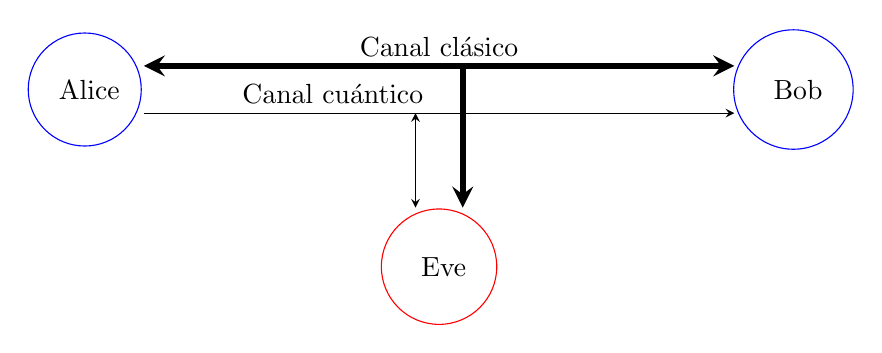
\begin{tikzpicture}[x=1.5cm, y=1.5cm]
    \node[circle,draw=blue] (v1) at (-3,0) {\ \ Alice\ \ };
    \node[circle,draw=blue] (v2) at (3,0) {\ \ \ Bob\ \ \ };
    \node[circle,draw=red] (v3) at (0,-1.5) {\ \ \ Eve\ \ \ };
    
    \draw[line width=0.8mm, {stealth}-{stealth}]  (-2.5,0.2) -- (2.5,0.2);
    \draw[line width=0.8mm, -{stealth}]  (0.2,0.2) -- (0.2,-1);
    
    \draw[-{stealth}]  (-2.5,-0.2) -- (2.5,-0.2);
    \draw[{stealth}-{stealth}]  (-0.2,-0.2) -- (-0.2,-1);
    
    \node at (0,0.2) [anchor=south] {Canal clásico};
    \node at (-0.9,-0.2) [anchor=south] {Canal cuántico};
\end{tikzpicture}
\end{center}
\caption{Esquema de distribución de clave cuántica.}
\label{fig:fig21}
\end{figure}

El primer paso del algoritmo es la elección de dos bases, como $\{\ket0,\ket1\}$ y $\{\ket+,\ket-\}$ y Alice procede a preparar una secuencia de bits. Para cada bit se elige aleatoriamente una de las bases para codificarlos, de manera que dicha codificación queda
\[\mathrm{bien\ }\begin{matrix}0\to\ket0\\1\to\ket1\end{matrix}\mathrm{,\ o\ bien\ }\begin{matrix}0\to\ket+\\1\to\ket-\end{matrix}\] 

en función de la base elegida. Tras la codificación, Alice envía a Bob la secuencia de qubits generada. Bob procede ahora a medir eligiendo, para cada qubit, una de las dos bases anteriormente citadas. Tras esta medición, tanto Alice como Bob hacen públicas las bases en las que la primera codificó y el segundo midió. Alrededor del 50\% de cada elección de estas bases coincidirá y los resultados asignados a estas elecciones se validan, mientras que el resto se desechan.

\begin{table}[htb]
\begin{tabular}{lll}
\rowcolor[HTML]{FFFFC7} 
Número del qubit & Base en la que codificó Alice & Base en la que midió Bob \\ 
\rowcolor[HTML]{FD6864} 
1                                & $\ket0,\ket1$                 & $\ket+,\ket-$            \\ 
\rowcolor[HTML]{9AFF99} 
2                                & $\ket0,\ket1$                 & $\ket0,\ket1$            \\ 
\rowcolor[HTML]{9AFF99} 
3                                & $\ket+,\ket-$                 & $\ket+,\ket-$            \\ 
\rowcolor[HTML]{FD6864} 
4                                & $\ket0,\ket1$                 & $\ket+,\ket-$            \\ 
\rowcolor[HTML]{9AFF99} 
5                                & $\ket+,\ket-$                 & $\ket+,\ket-$            \\ 
\rowcolor[HTML]{FD6864} 
6                                & $\ket+,\ket-$                 & $\ket0,\ket1$            \\ 
\rowcolor[HTML]{FD6864} 
7                                & $\ket+,\ket-$                 & $\ket0,\ket1$            \\ 
\rowcolor[HTML]{9AFF99} 
8                                & $\ket0,\ket1$                 & $\ket0,\ket1$            \\ 
\rowcolor[HTML]{9AFF99} 
9                                & $\ket0,\ket1$                 & $\ket0,\ket1$            \\ 
\rowcolor[HTML]{FD6864} 
10                               & $\ket0,\ket1$                 & $\ket+,\ket-$            \\ 
\rowcolor[HTML]{FFFFC7} 
...                              & ...                           & ...                      \\ 
\end{tabular}
\caption{Ejemplo de bases tomadas por Alice y Bob.}
\label{tab:tab21}
\end{table}

En el cuadro \ref{tab:tab21} se muestra un ejemplo de esta validación para los 10 primeros qubits de una secuencia. En verde aparecen los qubits para los que la base elegida por ambos coincidió y por tanto la medición de Bob arrojó el mismo resultado que la codificación de Alice. En rojo, por el contrario, aparecen aquellos cuyas bases no coincidieron y se descartan por no aportar información.

Ahora Alice y Bob pueden revelar una pequeña cantidad los valores obtenidos por cada uno, por ejemplo los $n$ primeros. Si todos esos valores coinciden, el canal es seguro y pueden utilizar el resto de los valores medidos no desvelados como clave. ¿Qué hubiera pasado si Eve hubiera intervenido el canal y hubiera tratado de medir los qubits antes de que lo hiciera Bob?

Al igual que Bob, Eve desconoce la base elegida por Alice para cada qubit, luego tendría que elegir una aleatoriamente  y realizar una medición. En el caso de escoger la misma que Alice (aunque Eve no podía tener la certeza hasta más tarde de haber acertado), no sólo podrá conocer el valor que codificó sino que además no está cambiando el estado del qubit y podrá reenviarlo a Bob inalterado. Esto ocurrirá en el 50\% de los casos; Sin embargo, en la otra mitad habrá elegido la base incorrecta modificando el estado del qubit y si Bob sí acierta con la base de Alice sólo tendrá un 50\% de posibilidades de medir el mismo valor que Alice codificó cuando debería serlo del 100\%.

Es así que Eve está introduciendo una variación en los estados en el 50\% de los qubits lo que supone que los valores de Alice y Bob diferirán en un 25\%. Si la cantidad de mediciones reveladas por ambos es de $n=20$ tras el intento de Eve de interceptar la comunicación, las probabilidades de no darse cuenta de la interferencia (no detectando ningún error) es de $0,75^{20}\approx0,32\%$. Tomando $n=30$ la probabilidad de pillar a Eve asciende a aproximadamente un 99,98\%, con lo que la certeza de garantizar la seguridad del canal es prácticamente absoluta con un tamaño de $n$ no necesariamente grande.

\section{Múltiples Qubits}

A lo largo de esta sección veremos cual es el comportamiento de un sistema cuántico cuando tenemos más de un qubit. Es aquí donde realmente podremos atisbar la capacidad de cómputo que tienen este tipo de máquinas.

En el física tradicional, si tenemos un sistema con $n$ partículas, cada una de ellas representada por un vector de dimensión 2, es el espacio vectorial que se genera es de dimensión $2n$. Esto se debe a que cada partícula se comporta de manera independiente y por tanto con ser capaces de modelizar el comportamiento individual de cada partícula tendremos representado todo el sistema. Es por ello que las dimensiones aumentan de manera lineal.

Sin embargo, esto no ocurre en mecánica cuántica. Las partículas ya no se comportan de manera independiente, si no que hay una dependencia entre ellas. Este efecto se llama \textbf{entrelazamiento} y entraremos en detalle posteriormente. 

Es por este motivo por el que no podemos modelizar los sistemas cuánticos con el comportamiento individual de cada partícula, si no que necesitaremos de una herramienta más potente, el \textbf{productor tensorial}.

\subsection{Producto Tensorial}

Supongamos que tenemos dos espacios vectoriales $\mathcal{V},\mathcal{W}$ de dimensiones $n$ y $m$ respectivamente. Entonces $\mathcal{V}\otimes\mathcal{W}$ es un espacio vectorial de dimension $n\times m$ y representa el producto tensorial de ambos espacios.

Además, supongamos que tenemos bases ortogonales para $\mathcal{V}$ y $\mathcal{W}$ dadas por:
\begin{equation}
\begin{split}
\mathcal{B}_v =\{\ket{v_i} |\ 1 \leq i \leq n \} \\
\mathcal{B}_w =\{\ket{w_j} |\ 1 \leq j \leq m \}
\end{split}
\end{equation}

Entonces una base $\mathcal{B}$ del espacio vectorial $\mathcal{V}\otimes\mathcal{W}$ se obtiene mediante el producto tensorial de los vectores de $\mathcal{B}_v$  y $\mathcal{B}_v$, es decir:
\begin{equation}
\mathcal{B} = \{\ket v\otimes\ket w|\ket v\in\B_v,\ket w\in\B_w\}
\end{equation}

Normalmente se aligera la notación y denotaremos $\ket{\phi}\otimes\ket{\psi}$ simplemente por $\ket{\phi}\ket{\psi}$ o incluso por $\ket{\phi\psi}$.

Por definición, el producto tensorial cumple las siguientes tres propiedades [\cite{nielsen2001quantum}]:
\begin{enumerate}
\item Dado un escalar z y un vector $\ket{v}$ de $\mathcal{V}$ y $\ket{w}$ de $\mathcal{W}$,\\
\begin{equation}
z(\ket{v}\otimes\ket{w})= (z\ket{v})\otimes\ket{w} = \ket{v}\otimes (z\ket{w})
\end{equation}

\item Para los vectores $\ket{v_1}$  y $\ket{v_2}$ de $\mathcal{V}$ y $\ket{w}$ de $\mathcal{W}$,\\
\begin{equation}
(\ket{v_1}+\ket{v_2})\otimes\ket{w}=\ket{v_1}\otimes\ket{w}+\ket{v_2}\otimes\ket{w}
\end{equation}

\item Para los vectores $\ket{v}$ de $\mathcal{V}$ y $\ket{w_1}$, $\ket{w_2}$ de $\mathcal{W}$,\\
\begin{equation}
\ket{v}\otimes (\ket{w_1}+\ket{w_2}) = \ket{v}\otimes\ket{w_1} +\ket{v}\otimes\ket{w_2} 
\end{equation}
\end{enumerate}

Hemos visto el producto tensorial aplicado a espacios vectoriales y hemos definido las propiedades que debe verificar un operador para ser considerado tensorial. Veamos cómo aplicaremos este operador en el caso de vectores, aunque lo haremos de una manera más general, definiendo el producto tensorial entre matrices. No olvidemos que un vector tiene una representación matricial como columna.

Sean $A$ y $B$ matrices con coeficientes complejos de dimensiones $m\times n$ y $p\times q$ respectivamente. Se verifica

\begin{equation}
A\otimes B=\left(\begin{matrix}
a_{11}B & \hdots & a_{1n}B \\
\vdots & \ddots & \vdots \\
a_{m1}B & \hdots & a_{mn}B
\end{matrix}\right)
\end{equation}

lo que supone que la matriz resultante $A\otimes B$ tiene dimensiones $mp\times nq$. Así, sean dos qubits, cuyos espacios vectoriales están representados respectivamente por la base ortonormal estándar $\{\ket0,\ket1\}$. Entonces, el nuevo espacio vectorial 
generado por ambos qubits tiene como base los vectores $\{\ket{00},\ket{01},\ket{10},\ket{11}\}$, es decir, un espacio de dimensión 4. Sin embargo, este ejemplo no es demasiado ilustrativo (pues $2^n = 2n$ si $n=4$).

Así que supongamos que añadimos un tercer qubit a nuestro sistema de dos qubits. Entonces el nuevo espacio vectorial tendrá dimensión 8 ($2^3$) y su base viene dada por los vectores $\{\ket{000},\ket{001},\ket{010},\ket{011},\ket{100},\ket{101},\ket{110},\ket{111}\}$.

Si repetimos estos cálculos pero utilizando la representación de la base como matri

% QUE NO SE TE OLVIDE INCLUIR QUE HAY ESTADOS CUANTICOS QUE NO SE PUEDEN EXPRESEAR COMO PRODUCTO TENSORIAL DE ESTADOS MÁS SIMPLES (COMO |00> + |11>) Y QUE SE DENOMINAN ENTRELAZADOS. DECIDE SI METER LAS CUENTAS DE SUPONGO QUE SI SE PUEDE Y JAJA NO SE PUEDE O DARLO POR SABIDO.

\section{Puertas cuánticas}

En computación clásica los bits son operados mediante una serie de puertas que son representadas como un circuito cableado. De igual modo tenemos puertas en el mundo cuántico. Dichas puertas tienen que verificar ser isomorfismos lineales unitarios; es decir, Si $U$ es la matriz asociada de dicho isomorfismo, se debe verificar que

\begin{equation}
UU^*=I
\end{equation}

donde $U^*$ es la matriz conjugada traspuesta de $U$. Una consecuencia inmediata de esta igualdad es que cualquier puerta cuántica es reversible, cosa que no ocurría con las clásicas. Además, por ser isomorfismo, el número de qubits de entrada coincidirá con el de salida.

\subsection{Puerta cuánticas de un qubit}

Vamos a proceder a hablar de algunas de las puertas cuánticas que cuentan con un solo qubit de entrada y salida más relevantes. Mostraremos la transformación realizada por cada una de ellas sobre los elementos de la base $\{\ket0,\ket1\}$, su expresión matricial y cómo se representan gráficamente sobre un circuito.

\[\begin{matrix}
\gatetwo{I}{\ket0}{\ket1} & \left(\begin{matrix}1&0\\0&1\end{matrix}\right) & \Qcircuit @C=1em @R=.7em {& \gate{I} & \qw}\\
\gatetwo{X}{\ket1}{\ket0} & \left(\begin{matrix}0&1\\1&0\end{matrix}\right) & \Qcircuit @C=1em @R=.7em {& \gate{X} & \qw}\\
\gatetwo{Y}{-\ket1}{\ket0} & \left(\begin{matrix}0&1\\-1&0\end{matrix}\right) & \Qcircuit @C=1em @R=.7em {& \gate{Y} & \qw}\\
\gatetwo{Z}{\ket0}{-\ket1} & \left(\begin{matrix}1&0\\0&-1\end{matrix}\right) & \Qcircuit @C=1em @R=.7em {& \gate{Z} & \qw}\\
\end{matrix}\]

Estas cuatro puertas son denominadas \textbf{puertas de \textit{Pauli}}. La primera de ellas se trata de la identidad que deja un estado cuántico invariable. $X$ es la puerta negación, dado un qubit $\ket\psi=\alpha\ket0+\beta\ket1$, tenemos que $X(\ket\psi)=\beta\ket0+\alpha\ket1$. $Z$ aplica un cambio de fase sobre $\ket1$ pero no varía las amplitudes (y por tanto tampoco las probabilidades de obtener $\ket0$ o $\ket1$ aplicando una medición). Por último, $Y$ es combinación de $X$ y $Z$ ($Y=ZX$).

Existen otras puertas de cambio de fase como $Z$ que denotamos de manera general por:

\[\begin{matrix}
\gatetwo{R_\theta}{\ket0}{e^{i\theta}\ket1} & \left(\begin{matrix}1&0\\0&e^{i\theta}\end{matrix}\right) & \Qcircuit @C=1em @R=.7em {& \gate{R_\theta}& \qw}
\end{matrix}\]

Nótese que $R_\pi=Z$. La puerta más relevante que veremos en esta sección es la \textbf{Puerta de \textit{Hadamard}}. Esta puerta es importante puesto que nos permite conseguir un estado en superposición de manera que las amplitudes de $\ket0$ y $\ket1$ produzcan equiprobabilidad en la medición. La describimos como:

\[\begin{matrix}
\gatetwo{H}{\dfrac{1}{\sqrt{2}}(\ket0+\ket1)}{\dfrac{1}{\sqrt{2}}(\ket0-\ket1)} & \left(\begin{matrix}\dfrac{1}{\sqrt{2}}&\dfrac{1}{\sqrt{2}}\\\dfrac{1}{\sqrt{2}}&-\dfrac{1}{\sqrt{2}}\end{matrix}\right) & \Qcircuit @C=1em @R=.7em {& \gate{H}& \qw}
\end{matrix}\]

Si esta puerta se aplica individualmente a cada uno de los $n$ qubits de un sistema con estado inicial $\ket{0\hdots0}$ obtenemos:

\begin{equation}
\dfrac{1}{\sqrt{2}}(\ket0+\ket1)\otimes\hdots\otimes\dfrac{1}{\sqrt{2}}(\ket0+\ket1)=\dfrac{1}{\sqrt{2^n}}\sum_{i=1}^{2^n-1}\ket i
\end{equation}

Esta última igualdad nos da una idea del poder que puede alcanzar el cómputo cuántico, pues hemos obtenido $2^n$ estados distintos en superposición. Cuando aplicamos la puerta de \textit{Hadamard} sobre $n$ qubits la denominamos \textbf{puerta de \textit{Walsh-Hadamard}} definida recursivamente como:

\[\begin{matrix}W_1=H,&W_{n+1}=H\otimes W_n\end{matrix}\]

En la figura \ref{fig:fig22} podemos ver un ejemplo sencillo de la aplicación de la puerta de \textit{Hadamard} sobre los 4 qubits de un sistema cuántico (o equivalentemente la aplicación de la puerta $W_4$). El estado del sistema tras la aplicación de dichas puertas es de 

\[\ket\psi=\dfrac{1}{4}\sum_{i=0}^{15}\ket i.\]

\begin{figure}[!htb]
\[\Qcircuit @C=1em @R=.7em {
\lstick{\ket{0}} & \qw & \qw & \gate{H} & \qw & \qw & \qw \\
\lstick{\ket{0}} & \qw & \qw & \gate{H} & \qw & \qw & \qw \\
\lstick{\ket{0}} & \qw & \qw & \gate{H} & \qw & \qw & \qw \\
\lstick{\ket{0}} & \qw & \qw & \gate{H} & \qw & \qw & \qw
}\]
\caption{Puertas de \textit{Hadamard} aplicadas a un sistema de 4 qubits.}
\label{fig:fig22}
\end{figure}

\subsection{Puertas cuánticas de más de un qubit}

La puerta de \textit{Walsh-Hadamard} está definida para más de un qubit; Sin embargo, puede ser expresada con producto tensorial de varias puertas de un solo qubit. No es el caso de las puertas que veremos en esta sección. En primer lugar presentamos la puerta \textbf{\textit{SWAP}} cuya función es intercambiar los estados de dos qubits. Su representación matricial es

\[\left(\begin{matrix}1&0&0&0\\0&0&1&0\\0&1&0&0\\0&0&0&1\end{matrix}\right)\mathrm{\ y\ en\ circuitos\ se\ representa\ como\ }
\Qcircuit @C=1em @R=1em {
& \qswap & \qw \\
& \qswap \qwx & \qw
}.\]

Un grupo de puertas de dos qubits muy relevante es el de las \textbf{puertas controladas}. Su funcionamiento consiste en tomar un primer qubit como control que permanecerá inalterado y un segundo al que se le aplicará una puerta $U$ o no en función del estado del primero. Su representación matricial por bloques viene dada por

\[C(U)=\left(\begin{array}{c|c}I&0\\\hline0&U\end{array}\right).\]

La más importante de ellas es $C(X)$, más conocida como \textbf{\textit{CNOT}} descrita por:

\[\begin{matrix}
\gatefour{\mathrm{CNOT}}{\ket{00}}{\ket{01}}{\ket{11}}{\ket{10}} & \left(\begin{matrix}1&0&0&0\\0&1&0&0\\0&0&0&1\\0&0&1&0\end{matrix}\right) & \Qcircuit @C=1em @R=1em {& \ctrl{1} & \qw \\
& \targ & \qw}
\end{matrix}\]

donde $\bullet$ denota el qubit de control y $\oplus$ el qubit negado (si procede). Como vemos, la puerta $X$ se aplica sobre el segundo qubit si el estado del primero es $\ket1$.

Existen puertas controladas en las que intervienen más de dos qubits como la \textbf{\textit{CCNOT}} o \textbf{puerta de \textit{Toffoli}}. Se trata de una puerta de 3 qubits, los dos primeros de control que permanecen inalterados y el último al que se le aplica una puerta $X$ siempre y cuando los dos primeros sean $\ket1$. Para simplificar, mostramos su matriz por bloques y su representación en circuito:

\[\begin{matrix}
T=\left(\begin{array}{c|c|c}I&0&0\\\hline0&I&0\\\hline0&0&X\end{array}\right) & \Qcircuit @C=1em @R=1em {& \ctrl{1} & \qw \\
& \ctrl{1} & \qw \\
& \targ & \qw}
\end{matrix}\]

Esta puerta tiene una importancia adicional porque con ella podemos emular las puertas clásicas \textbf{NOT} y \textbf{AND} que constituyen un conjunto universal que permiten construir cualquier circuito clásico.

\begin{equation}
\begin{split}
T\ket{1,1,x}=\ket{1,1,\neg x} \\
T\ket{x,y,0}=\ket{x,y,x\wedge y}
\end{split}
\end{equation}

En la ecuación anterior se muestran las construcciones de dichas puertas respectivamente. Nótese que $T$ permite generar cualquier circuito clásico pero no afirmamos tal cosa de los circuitos cuánticos (de hecho no se verifica esta segunda proposición). La generación de estas puertas ayudó a probar a Deutsch que cualquier función clásica puede ser fabricada a partir de una puerta cuántica reversible [\cite{deutsch1985quantum}]. Incluso Bernstein y Vazirani concretaron una \textbf{máquina cuántica universal de Turing} [\cite{bernstein1997quantum}].

Según lo que acabamos de ver, dada una función clásica $\function{f}{\{0,1\}^m}{\{0,1\}^k}$ existe un \textbf{\textit{array} de puertas} $U_f$ que implementa $f$ en un circuito cuántico. Se verifica que $U_f\ket{x,y}=\ket{x,y\oplus f(x)}$ donde $x$ denota un elemento de $m$ bits, $y$ de $k$ bits y $\oplus$ es el operador lógico XOR.

\begin{figure}[!htb]
\[\Qcircuit @C=1em @R=.7em {
\lstick{\ket{x}}& \multigate{1}{U_f} & \qw & \qw & \qw & \qw & & \lstick{\ket{x}} \\
\lstick{\ket{y}}& \ghost{U_f}        & \qw &     &     &     & & \lstick{\ket{y\oplus f(x)}}
}\]
\caption{Representación en un circuito cuántico de un \textit{array} de puertas cuántico.}
\label{fig:fig23}
\end{figure}

Véase que $U_fU_f\ket{x,y}=U_f\ket{x,y\oplus f(x)}=\ket{x,y\oplus f(x)\oplus f(x)}=\ket{x,y}$. Luego $U_fU_f=I$ y por lo tanto verifica que es unitaria. Para calcular $f(x)$ basta con aplicar $U_f\ket{x,0\hdots0}$ cuyo resultado será $\ket{x,f(x)}$.

Sin embargo esto no parece suponer una gran ventaja respecto la computación clásica. Pero, ¿y si pudiéramos obtener todos los valores $f(x)$ para cada $x\in\{0,1\}^m$ con una sola aplicación de $U_f$? Esto constituye una mejora de complejidad exponencial a constante y lo conseguimos aplicando una puerta de \textit{Hadamard} a cada uno de un total de $m$ qubits (es decir, aplicar $W_m$), además de preparar otros $k$ qubits en estado $\ket0$ tal y como muestra la figura \ref{fig:fig24}.

\begin{figure}[!htb]
\[\Qcircuit @C=1em @R=.7em {
\lstick{\ket{0\overset{m}\hdots0}}& \gate{W_m} & \multigate{1}{U_f} & \qw \\
\lstick{\ket{0\overset{k}\hdots0}}& \qw        & \ghost{U_f}        & \qw
}\]
\caption{Ejemplo del poder del paralelismo cuántico aplicado a un \textit{array} de puertas.}
\label{fig:fig24}
\end{figure}

Analíticamente, por la linealidad de $U_f$, tenemos:

\begin{equation}
\begin{split}
U_f(W_m(\ket{0\overset{m}\hdots0})\otimes\ket{0\overset{k}\hdots0})&=U_f\left(\dfrac{1}{\sqrt{2^m}}\sum^{2^m-1}_{i=0}\ket{i,0\overset{k}\hdots0}\right)=\\
&=\dfrac{1}{\sqrt{2^m}}\sum^{2^m-1}_{i=0}U_f\ket{i,0\overset{k}\hdots0}=\dfrac{1}{\sqrt{2^m}}\sum^{2^m-1}_{i=0}\ket{i,f(i)}
\end{split}
\end{equation}

No obstante, todo esto no es tan maravilloso como parece. Recordemos que sólo podemos obtener información de un estado cuántico mediante la medición y, que tras esta, el estado que obtengamos será el mismo al que colapsará el sistema y será único, con lo que perdemos este poder de \textbf{paralelismo cuántico} que acabábamos de obtener. Antes de medir, debemos aplicar algunas técnicas adicionales, alejadas de la computación clásica como por ejemplo amplificar las amplitudes (y con ellas las probabilidades de medir ese estado) de los valores de mayor interés.

\subsection{Teorema de no clonación}

\begin{thm} \textbf{Teorema de no clonación}
\end{thm}

% Introducción al testing. Mutation testing. ¿Quantum Error Correction?
\chapter{Introducción al Testing}
Uno de los pilares fundamentales de este trabajo es el testing, más concretamente una técnica muy usada en este área, el \textit{mutation testing}. Por ello, a lo largo del siguiente capítulo daremos 
unas pinceladas muy básicas sobre en qué consiste el testing y hablaremos más en profundidad  de la técnica mencionada previamente.

\section{¿Qué es el Testing?}

El \emph{testing} es una disciplina de la \textit{Ingeniería del Software} orientada a aumentar la calidad y la fiabilidad de un programa. Su principal objetivo es encontrar errores en el software para de esta manera poder corregirlos.

Hay que tener muy en cuenta que demostrar el correcto funcionamiento de un programa es un problema no decidible, y por tanto este no es el objetivo del testing. En palabras de Edsger Wybe Dijkstra [\cite{dijkstra1972chapter}], el testing permite encontrar errores pero, sin embargo, no permite demostrar la ausencia de ellos.

A la hora de encontrar un fallo en el software, hay 3 términos que hay que tener muy claros para poder describir con precisión la naturaleza del fallo en cuestión. Se introducen los términos en inglés, pues su traducción puede inducir a confusiones no deseadas:
\begin{itemize}
\item \emph{Fault}: es el termino que se utiliza para indicar un defecto estático en el código del programa que está siendo testeado.
\item \emph{Error}: se corresponde con un estado incorrecto del programa durante la ejecución del mismo.
\item \emph{Failure}: se produce cuando el comportamiento externo del programa es incorrecto respecto a los requisitos establecidos para este.
\end{itemize}

La unidad u objeto fundamental del testing son los \emph{tests}. Un test se constituye principalmente de dos componentes:
\begin{itemize}
\item \emph{Inputs}: son los valores que se necesita aportar al programa para que se ejecute de la forma concreta que está siendo testeada.
\item \emph{Outputs}: se corresponde con el resultado que producirá el programa en caso de que su comportamiento sea correcto.
\end{itemize}

Como el software puede constar de múltiples funcionalidades, va a ser necesario contar numerosos de tests para poder verificarlo correctamente. A un conjunto de test se lo conoce como \textit{test suite}. 

Por otro lado, los programas suelen ser inmensamente extensos, y comprobarlos completamente no es viable. El número de inputs  que puede aceptar un programa puede ser ``infinito''. Pensemos por ejemplo en un compilador de Java. Potencialmente, los inputs que puede recibir el compilador no son sólo todos los programas Java, si no cualquier cadena de caracteres. La única limitación viene impuesta por el máximo tamaño de archivo que acepta el \textit{parser} del compilador. Por eso se dice que el número de inputs es ``infinito''. [\cite{ammann2016introduction}]

Siguiendo la literatura que acabamos de mencionar, la manera de solucionar este problema es introduciendo unos criterios que permitan al testeador diseñar tests eficaces, es decir, tets que potencialmente sean más propensos a encontrar \textit{faults} en el código. Estos criterios son:
\begin{itemize}
\item \emph{Requisito de Test}: es un ``artefacto'' concreto del software que se debe cumplir durante el proceso de testing.
\item \emph{Requisitos de Cobertura}: son un conjunto de reglas que debe cumplir un \textit{test suite} para que se verifiquen todos los requisitos de test. Existen diversos tipos de cobertura basados en: grafos, lógica proposicional, dominio de los inputs ...
\end{itemize}

Una vez que se tienen unas nociones básicas del testing, podemos mover el foco hacia la rama del testing que realmente concierne a este trabajo. Igual que un \textit{test suite} nos va a permitir
encontrar fallos en un programa, es igual de interesante ver la eficiencia de dicho \textit{test suite}. Imaginemos que tenemos un programa con una serie de \emph{faults} en el código. Puede ocurrir que si se diseña un \textit{test suite} sobre unos requisitos de test pobres, dicho test suite no de lugar a ningún \emph{failure}, y esto no se debe a que el programa funcione correctamente,si no a que el conjunto de test no es bueno.

Así nace el \textit{mutation testing}, un técnica desarrollada con el objetivo de poder comprobar la eficacia de los tests.

\section{Mutation Testing}

% Mutation Testing aplicado a computación cuántica
\chapter[Mutation Testing en computación cuántica]{Mutation Testing aplicado a la computación cuántica}
Una vez vistos  los principales conceptos e ideas detrás de  mutation testing, podemos tratar de abordar el problema de aplicar esta técnica a software cuántico. En este capítulo presentaremos un marco  general para mostrar  cómo se podrían adaptar las nociones de mutation testing que se utilizan en el mundo de la programación clásica al mundo cuántico para, posteriormente, centrar el desarrollo del capítulo en torno a los dos lenguajes de programación cuánticos que consideramos en  este trabajo: \textit{Qiskit} y \qsh.

\section{Diseño de operadores de mutación}

La  tarea más crítica que conforma el diseño de un marco de mutation testing para un lenguaje concreto, sea este cuántico o no, consiste en  diseñar  los operadores de mutación. Tal y como se vió en el capítulo anterior, los operadores de mutación debe modelar errores comúnmente cometidos por los programadores. Aquí se encuentra la primera dificultad con la que nos encontramos a la hora de diseñar una serie de operadores en el entorno cuántico.

Los lenguajes de programación cuánticos se han empezado a desarrollar durante los últimos años y, aunque han ido ganado notoriedad con el paso del tiempo, todavía no se están realizando grandes proyectos con este tipo de lenguajes. Esto puede deberse a que el desarrollo de sistemas cuánticos está evolucionando a un paso lento y el mayor computador cuántico del que se tiene conocimiento público a día de hoy, desarrollado por IBM, consta de tan sólo $53$ qubits. Por tanto, pese a que un desarrollador de software puede contar a nivel de simulador con el número de qubits que considere necesario, es posible que no pueda ejecutar dicho código en una máquina física y disfrutar de la capacidad de cómputo que ofrecen estos sistemas.
%
Si hacemos una analogía con la computación clásica,
la tarea de identificar los errores más comunes cometidos por un programador es relativamente sencilla para lenguajes clásicos como \textit{Java}, C\texttt{++} o \textit{Python}, dado que existen infinidad de repositorios de código donde poder realizar un estudio sobre qué métodos u operadores son más utilizados. Además,  se cuenta con múltiples plataformas de preguntas y respuestas donde poder inspeccionar cuales son los errores más habitualmente cometidos para cada lenguaje. Sin embargo, esto no ocurre para lenguajes de computación cuántica. Si bien cada vez aparecen más repositorios con código cuántico, así como  plataformas donde los programadores pueden exponer sus problemas durante el desarrollo, todavía no tienen la cantidad de información suficiente para permitir un estudio a media escala sobre el código cuántico que permita identificar aquellos errores que son lo más adecuados para ser modelados como operadores de mutación. Más adelante se detalla como se decide abordar este problema para los lenguajes \textit{Qiskit} y \qsh.

Este no es el único problema que tiene la aplicación de mutation testing en código cuántico. El otro gran inconveniente es la especificación de los test, más en concreto la especificación de las entradas.

\section{Especificación de inputs cuánticos}

Una vez que se cuenta con el diseño de los operadores de mutación, la obtención de mutantes para un programa cuántico no difiere del proceso análogo para lenguajes de programación clásicos. Dicho proceso consiste tan sólo en buscar y reemplazar una cadena del código siguiendo las reglas concretas del operador de mutación que se desea aplicar.

Tras obtener el conjunto de mutantes, el siguiente paso a realizar es aplicar el conjunto de tests a dichos mutantes. Recordemos que un test se compone  de unos valores de entrada, inputs, y de los  valores de salida esperados, outputs. 
%
Aunque a simple vista pueda parecer que este proceso es sencillo, cuenta con una serie de dificultades. Una de ellas es obtener los valores que provoquen que se alcance el estado del programa que se quiere testear. Estos valores son conocidos como \emph{valores de prefijo}. De la misma forma, los valores que debe recibir el programa tras alcanzar el estado que se desea testear y que nos permiten terminar la ejecución del programa o ver los resultados, conocidos como \emph{valores de postfijo}, también presentan una complicación a la hora de diseñar los tests. Obtener estos valores de prefijo y postfijo suponen una tarea extra para el encargado de desarrollar el conjunto de tests y es necesario llevarla a cabo tanto en programación clásica como en programación cuántica. Sin embargo, con este último tipo de programación surge un nuevo problema que no se tiene con los lenguajes de programación clásicos.
\begin{figure}[htb!]
\begin{lstlisting}[language=c++]
using (register = Qubit[2]) {

	//LLamar al metodo y guardar el output
	let(output) =  method(register);

	ResetAll(register);
	
	return output;
}
\end{lstlisting}
\begin{lstlisting}[language=c++]
using (register = Qubit[2]) {

	//Inicializar los qubits al estado deseado
	X(register[0]);
	H(register[1]);
	
	//LLamar al metodo y guardar el output
	let(output) =  method(register);

	ResetAll(register);
	
	return output;
}
\end{lstlisting}
\caption{Llamada a method con inicialización de qubits al estado deseado.}
\label{fig:code42}
\end{figure}

En algunos de los lenguajes de programación cuánticos, como es el caso de \textit{Qiskit} y \qsh, se tienen tipos primitivos pertenecientes al paradigma de la programación clásica como enteros o booleanos. Estos tipos no suponen ningún problema si son necesarios como entradas de un test, pues son fácilmente declarables independientemente del lenguaje. Sin embargo, con la computación cuántica aparece un nuevo tipo: el qubit. 
%
Generalmente, cuando se declara un qubit, comienza inicializado al valor $\ket{0}$. Si el encargado de diseñar los test desea comprobar el funcionamiento de cierto método con un qubit que se encuentre en un estado diferente al $\ket{0}$, debe ser él el encargado de transformar el qubit al estado deseado mediante la aplicación de puertas cuánticas. Por tanto, el testeador necesita diseñar para cada test un circuito cuántico que se encargue de llevar al estado deseado cada qubit que se vaya a utilizar como entrada de un test. Esto supone añadir un grado de complejidad a la obtención de valores de prefijo.

Para ver con más claridad el problema que acabamos de presentar, veamos un ejemplo. Supongamos que tenemos el  código, en el lenguaje \qsh, que se presenta en la parte superior de la figura~\ref{fig:code42}.
%
Adicionalmente, supongamos que se quiere realizar un test donde los 2 qubits del registro estén inicializados a los valores $\ket{1}$ y $\tfrac{1}{\sqrt{2}}(\ket{0}+\ket{1})$, respectivamente. Entonces se 
debe añadir código al código anterior para representar estas inicializaciones. El resultado de esta inclusión aparece en la parte inferior de la figura~\ref{fig:code42}.
%
Por tanto, el testeador debe ser capaz de crear la secuencia de puertas que transforme cada qubit que se vaya a utilizar como input del test al estado cuántico deseado y esta secuencia se debe incluir dentro del código que se quiere testear.

Una vez que ya sabemos cómo se pueden generar los mutantes y cómo se pueden diseñar los tests, sólo falta decidir cuando hemos matado a un mutante. De nuevo aparece una dificultad añadida para esta tarea cuando trabajamos en el mundo cuántico.

\section{Decisión de la muerte de un mutante}

Tal y como se vio en el capítulo anterior, la manera más habitual de decidir si un mutante muere o no es comparando los outputs de la ejecución del mutante con los del programa original. Si intentamos llevar esta idea hacia la programación cuántica aparece de inmediato un inconveniente.

Los programas cuánticos son, en su mayor parte, probabilistas. Esto se debe a que están basados en el uso de qubits y, como ya se ha visto previamente, una medición de un qubit arroja dos posibles resultados con cierta probabilidad. Por lo tanto, en el momento en que se realice una medición, automáticamente el programa pasará a ser no determinista (dando por hecho que el resultado  obtenido en la medición es usado posteriormente). Para ilustrar este problema, véase el código de la figura~\ref{fig:code43}.

En este sencillo ejemplo simplemente transformamos un qubit que se encuentra en el estado $\ket{0}$ al estado $\tfrac{1}{\sqrt{2}}(\ket{0}+\ket{1})$ mediante una puerta \emph{Hadamard}. En dicho estado, el qubit tiene las mismas probabilidades de arrojar como resultado $\ket{0}$ o $\ket{1}$ al realizar una medición sobre él. La variable de salida \textit{output} depende del resultado de esta medición. Es obvio que distintas ejecuciones de este programa darán resultados diferentes. Este no-determinismo supone un inconveniente para realizar testing, pues un mismo test puede ser correcto para algunas ejecuciones de un programa y erróneo para otras. En particular, para mutation testing, no va a ser suficiente con ejecutar una vez el programa original y el mutante y comparar las salidas. En el marco que presentamos en esta memoria, se han tenido en cuenta dos alternativas que solventan este problema: realizar múltiples ejecuciones del programa o aprovechar las ventajas de trabajar con un simulador. Vamos a ver con detalle estas dos soluciones.
\begin{figure}[t]
\begin{lstlisting}[language=c++]
using (register = Qubit[1]) {
	
	mutable output = 0; 
	
	H(register[0]);
	let res = M(q0);
	
	if(res = One) {
		output = 1:
	}

	ResetAll(register);
	
	return output;
}
\end{lstlisting}
\caption{Ejemplo de superposición de estados.}
\label{fig:code43}
\end{figure}

\subsection{Valoración estadística de los outputs}

Una primera manera de abordar este problema consiste en realizar un estudio estadístico de los resultados. Para ello, se deberá ejecutar múltiples veces el programa original y, de igual manera, el mutante. El número de veces que se ejecutan estos programas es decidido por el encargado de testear, sabiendo que a medida que se aumenta el número de ejecuciones aumenta la fiabilidad del resultado. 

También es tarea del testeador decidir como comparar las salidas. Supongamos que un programa da como salida una tupla. Podemos entender dicho output como un {\it todo} y por tanto un mutante moriría si la tupla de salida no coincide íntegramente con la tupla retornada por el programa original. Pero también podemos entender dicha tupla como valores independientes. En ese caso, el el testeador debe distinguir cuantos elementos de las tuplas devueltas por el mutante y el programa original deben coincidir para matar o no a dicho mutante. Una vez que se decide como comparar las salidas y se ejecutan los programas correspondientes numerosas veces, hay que decidir una métrica estadística que nos permita dictaminar que mutantes mueren con un cierto valor de confianza. La métrica decidida en este trabajo se detalla en el siguiente capítulo.

\subsection{Estado interno del simulador}
\label{subsec:subsec432}
Una segunda forma que nos permite solucionar el inconveniente del no determinismo en la computación cuántica es aprovechar el uso del simulador. Hoy en día, el acceso a un máquina cuántica es realmente limitado. Por ello, la mayor parte de los lenguajes de programación cuánticos han sido diseñados para ser ejecutados en una máquina tradicional. Esto se traduce en que los programas cuánticos corren sobre un simulador y, por lo tanto, los estados de los qubits están siendo simulados y almacenados en bits corrientes. Es por ello que, al menos en el caso de \textit{Qiskit} y \qsh, se pone a disposición del programador herramientas que permitan interaccionar con el simulador. Una de estas herramientas posibilita mirar las amplitudes de los qubits en el simulador sin alterar el estado de estos. Esto en el mundo cuántico real no es posible, pues al observar el estado de un qubit, como ya bien sabemos, colapsa. Sin embargo, en simulación podemos hacer uso de esta herramienta para comparar las salidas de nuestros test de una manera muy eficiente. Decimos que un mutante muere si el estado interno de los qubits tras la ejecución es diferente al estado interno del programa original. Nos gustaría recalcar que somos conscientes de que esta aproximación se puede ver, legítimamente, como {\it hacer trampas}. Sin embargo, consideramos que es adecuada para analizar programas cuánticos a la hora de detectar {\it faults} en los mismos, incluso teniendo en cuenta que, finalmente, se ejecutarán en un ordenador cuántico donde no será posible hacer esta trampa.

Como no podría ser de otra forma en el mundo cuántico, hay una complicación adicional. Si nos limitamos a comprobar la igualdad entre dos qubits estaremos sopbrepasando el poder de distinción real que tenemos en el mundo cuántico. Por ello, debemos plantearnos la pregunta: ¿Cuando dos qubits son iguales?

Por un lado, en mecánica cuántica no se tienen en cuenta los cambios de \textit{fase globales} y consideramos que dos qubits son iguales módulo un cambio de fase, es decir, $\ket{\phi} =e^{i\theta}\ket{\phi}$. Esto se debe a que el operador de proyección es el mismo. Por tanto, las probabilidades que arrojan a la hora de medir son las mismas.

Además, los qubits que difieren por un cambio de \textit{fase relativo} de la forma: $\ket{\phi}= \alpha\ket{0} + e^{i\theta}\beta\ket{1}$ tienen las mismas probabilidades de medir $\ket{0}$ o $\ket{1}$ independientemente de la fase $\theta$ elegida (recordemos que $e^{i\theta}$ tiene modulo unidad).

Por lo tanto, a nivel de simulación, debemos considerar las probabilidades de medir $\ket{0}$ o $\ket{1}$ como factor para determinar si dos qubits son o no iguales.


\section{Mutation Testing en \textit{Qiskit} y \qsh}

En este capítulo hemos analizado  los principales inconvenientes que hemos encontrado a la hora de trasladar las ideas del mutation testing al mundo cuántico. Veamos ahora como se han desarrollado estos conceptos para los dos lenguajes que se consideran en este trabajo.

En esta última sección del capítulo vamos a centrarnos principalmente en el proceso llevado a cabo para el diseño de los operadores de mutación. Tanto la especificación de los inputs para los test, como la resolución de las muertes de los mutantes se detallarán en el siguiente capítulo, pues incide de manera más directa en el diseño del sistema desarrollado.

La primera decisión importante que se tuvo que realizar es decir qué elementos del lenguaje  eran candidatos a ser mutados. Tanto \textit{Qiskit} como \qsh\ son lenguajes que tienen una serie de métodos cuánticos, pero también están dotados de elementos clásicos como pueden ser bucles, sentencias condicionales o tipos primitivos básicos. Como mutation testing ya ha sido aplicado a este último tipo de elementos, se decidió orientar el trabajo al mundo cuántico y, por tanto, sólo se han tenido en cuenta como candidatos a operadores de mutación aquellos elementos puramente cuánticos.

Para el lenguaje \textit{Qiskit} se ha tenido en cuenta principalmente el intercambio de puertas cuánticas. De hecho, se consideró que era altamente probable que un programador confundiese dos puertas cuánticas y cometiese este tipo de error.

En el caso de \qsh\ también se consideró este tipo de operador de mutación pero, además, se añadió un nuevo tipo de operador. En este lenguaje hay una serie de constantes que son de naturaleza puramente cuántica. Por un lado, tenemos los resultados al realizar una medición, que vienen dados por las constantes \textit{Zero} y \textit{One} y, por otro lado, las constantes relativas a los operadores de Pauli: \textit{PauliX}, \textit{PauliY} y \textit{PauliZ}. Estas constantes se utilizan a la hora de especificar sobre qué eje se desea medir o a la hora de aplicar una rotación, entre otros. Se ha considerado como operador de mutación el intercambio de \textit{Zero} por \textit{One} y viceversa, así como cualquier intercambio dentro de los operadores de Pauli.

Por último, a muchos de los métodos de \qsh\ se les puede aplicar el functor \textit{Adjoint}, que proporciona la versión adjunta del método. Se ha considerado también como mutación que al programador se le olvide aplicar dicho functor.

% Gestión, planificación y desarrollo del proyecto de software
\chapter[Gestión, planificación y desarrollo del software]{Gestión, planificación y desarrollo del proyecto de software}
Ya hemos introducido las bases del \textit{testing}, de la computación cuántica y de las pruebas de mutación aplicada a la misma. Estamos en disposición de hablar del \textit{software} realizado y que trabaja sobre todos estos conocimientos.

\section{Gestión del proyecto}

En primer lugar vamos a tratar acerca de todo el proceso de gestión del proyecto, desde la organización como equipo, hasta herramientas y \textit{software} utilizado para el desarrollar el código y la memoria.

\subsection{Gestión de equipo}

La gestión del equipo es sencilla, en principio los dos miembros del grupo contamos con el mismo poder para la toma de decisiones y por tanto, dichas decisiones han de tomarse de manera consensuada. Si bien es cierto que, según la actividad, alguno de los miembros puede estar más involucrado en ella y es razonable que sus argumentos tenga un mayor peso.

Además, en caso de decisiones clave siempre teníamos una segunda opinión, correspondiente a nuestro tutor, que por tanto ha formado parte también de la toma de las mismas. Hemos tratado de involucrarnos por igual en todas las fases y tareas del TFG con, tal vez, algunas excepciones. Veremos a continuación de forma detallada la contribución de cada uno al trabajo.

\subsection{Contribución al proyecto de Luis Aguirre}
% Al menos dos páginas

\subsection{Contribución al proyecto de Javier Pellejero}
% Al menos dos páginas

\subsection{Gestión de configuración}

Hablemos ahora de todas las herramientas y elementos de \textit{software} utilizados para el proyecto. Empezando por esta memoria, al estar realizada en \LaTeX, hemos necesitado programas para su edición y compilación. Ambos componentes del grupo hemos utilizado como distribución \textit{MiKTeX}, mientras que como editor hemos usado \textit{Texmaker}.

En cuanto al \textit{software}, el grueso del programa está realizado en \textit{Java} y es utilizado como gestor y editor del mismo la plataforma \textit{Eclipse} usando como herramienta de desarrollo la octava versión \textit{Java SE Development Kit} (JDK) de \textit{Oracle}.

El programa principal debe realizar una serie de test sobre los lenguajes de computación cuántica \qsh\ y \textit{Qiskit}. En el caso del primero, permite ser llamado desde \csh\ y {Python}, siendo más común utilizar el primero. En el caso del segundo, más que un lenguaje en sí mismo, es un marco de trabajo que engloba varias librerías que se ejecutan sobre \textit{Python}. Se opta por dejar \csh\ de lado, puesto que \textit{Python} es el lenguaje en común de ambos, y que nuestro programa principal, mediante una llamada a sistema, ejecute un programa en dicho lenguaje.

Este programa cambia con cada ejecución y es el programa en \textit{Java} principal quien debe escribirlo. Sin embargo, se han de escribir archivos adicionales en \textit{Python} que contienen funciones útiles y siempre necesarias y para ello se emplea un programa de edición sencillo como \textit{Notepad++}, además de \textit{Jupyter Notebook}, usando la distribución \textit{Anaconda}, para verificar que nuestras funciones escritas tanto por nosotros como por el programa funcionan correctamente.

Para el correcto funcionamiento del programa en su conjunto, se necesitan una serie de requisitos.

\begin{itemize}
\item Una máquina virtual capaz de ejecutar \textit{Java} como \textit{Java Runtime Environment} (JRE).
\item \textit{Python} 2 o 3. (Se recomienda \textit{Python} 3).
\item La librería de \textit{Python} \textit{func-timeout} de Tim Savannah bajo licencia LGPLv3 accesible en \textbf{https://github.com/kata198/func\_timeout/blob/master/LICENSE}. Se adjunta en el repositorio del proyecto.
\item \qsh\ (sólo si se realizaran test con este lenguaje cuántico).
\item \textit{Qiskit} (sólo si se realizaran test con este lenguaje cuántico).
\end{itemize}

En cuanto a la organización y distribución de nuestro código, hemos elegido \textit{Github}. Además de ser un excelente gestor de versiones, tiene el programa (para el sistema operativo\textit{Windows}) \textit{Github Desktop}, una interfaz sencilla para subir y gestionar el código. En el repositorio existen dos carpetas principales en el directorio raíz:

\begin{itemize}
\item \textbf{tex}: que almacena el código \LaTeX.
\item \textbf{src}: que almacena el código, tanto \textit{Java} como \textit{Python}
\end{itemize}

Además existen otras carpetas de menor relevancia con contenidos como ejemplos en los dos lenguajes cuánticos tratados, presentaciones, además de encontrarse en la raíz principal la \textbf{licencia MIT}.

Como veremos, este programa no sólo puede ser realmente utilizado por cualquier interesado en realizar pruebas de mutación sobre programas cuánticos, sino que pueden ser integradas una serie de funcionalidades adicionales en el mismo. Por ello hemos optado por esta licencia, que posiblemente sea la de menor número de restricciones. Cualquiera puede tomar el proyecto y modificarlo, incluso para uso comercial.

\section{Planificación}

La planificación del proyecto puede dividirse en dos aspectos: uno desde el punto de vista temporal que incluye el proceso de investigación, \textit{software} y la realización de la memoria; y otro desde el punto de vista del modelo de proceso elegido para el \textit{software}.

\subsection{Planificación temporal}

Para planificar este Trabajo de Fin de Grado es importante entender que, como alumnos del doble grado en ingeniería informática y matemáticas, debemos realizar un TFG por grado. Nuestra idea inicial es que ambos trabajos estuvieran relacionados y ya en julio contactamos con nuestro tutor y conocíamos el tema de los mismos.

Dejamos constancia de que en el caso del TFG de matemáticas, dichos trabajos eran individuales aunque ambos alumnos tratamos un tema común que es el de introducirnos en la computación cuántica con una sólida base matemática y con alguna pincelada de conocimiento en mecánica cuántica. Además, cada uno introduce un lenguaje de programación cuántico: \qsh\ en el caso de Luis Aguirre y \textit{Qiskit} en el caso de Javier Pellejero.

Por tanto, se puede argumentar que este trabajo tiene sus cimientos en los dos realizados por cada miembro del grupo para el grado de matemáticas. Explicado esto, empezaremos por enumerar una serie de fases de planificación que incluye todos los trabajos.

\begin{enumerate}
\item \textbf{Proceso de investigación}. Puesto que se trata de una serie de conocimientos totalmente nuevos para nosotros y con una complejidad considerable, es importante dotar a esta fase de una duración prolongada. Decidimos establecer como límite para esta fase finales de enero coincidiendo con el fin de exámenes del primer cuatrimestre. En el segundo, ninguno de los integrantes del grupo tiene otras asignaturas, así que hay tiempo suficiente para el resto de fases.
\item \textbf{Desarrollo del \textit{software}}. Una vez familiarizados con la teoría de la computación cuántica y de pruebas de mutación, estamos en condiciones de comenzar nuestro programa. En las siguientes páginas se dará más detalle del mismo. En cuanto al tiempo, estimamos unos dos meses, febrero y marzo, para realizarlo.
\item \textbf{Memorias individuales del TFG del grado de matemáticas}. Por lo comentado anteriormente, es consecuente realizar primero estas memorias pues su contenido sirve de base para desarrollar esta misma. Se estable que el tiempo marcado por el mes de abril es apropiado para realizarla.
\item \textbf{Memoria del TFG del grado en ingeniería informática}. Siguiente tarea a efectuar. Prevista para el mes de mayo.
\item \textbf{Revisión}. Se establece el mes de junio para ultimar memorias, perfección del \textit{software} o cualquier otra tarea que pudiera no estar acabada.
\end{enumerate}

Aclaramos que estas fechas son orientativas. Como veremos a continuación, nuestro modelo de proceso del \textit{software} se asemeja a un \textbf{desarrollo evolutivo ágil}, concretamente al denominado \textbf{\textit{eXtreme Programming}} (XP) y sus principios pueden aplicarse también a toda la planificación anterior. Puesto que el tiempo no parece un problema determinante, no seremos estrictos con las fases anteriormente mencionadas.

\subsection{Modelo de proceso}

Acabamos de comentar el modelo en el que se basa nuestro desarrollo del programa. Creemos poder dar algunos buenos argumentos de por qué es una buena decisión. Al contar con un grupo de tan solo dos integrantes, la comunicación entre ambos es clara, concisa y rápida, no sólo entre nosotros sino también con el tutor (al que podemos asignar el rol de cliente), lo que ayuda a prevenir malentendidos que acaban en errores y problemas difíciles de vaticinar aún con un proceso de desarrollo pesado con una planificación más exhaustiva como el proceso unificado.

Otro factor a tener en cuenta es que, si bien los conceptos sobre los que trata nuestro programa no son elementales, no es excesivamente complejo el hecho de implementarlos. Además, al ser un área de la computación en el que no se ha investigado aún en exceso, puede surgir en cualquier momento la necesidad de cambios o implementar nuevas funcionalidades.

El uso de XP facilita este último hecho, pues intercala continuamente diseño y desarrollo de manera evolutiva e iterativa. En nuestro caso, es muy importante disponer de una versión ejecutable del programa desde el momento que esté desarrollada la primera funcionalidad, lo cual hemos logrado. Para ello, diseñamos una vista, le damos forma mediante código y la ensamblamos con la lógica. Antes de continuar una nueva vista, nos aseguramos que la funcionalidad implementada tiene una correcta actividad para evitar el encadenamiento de errores.

%------- Figura iteración XP
\begin{figure}[!htb]
\begin{center}
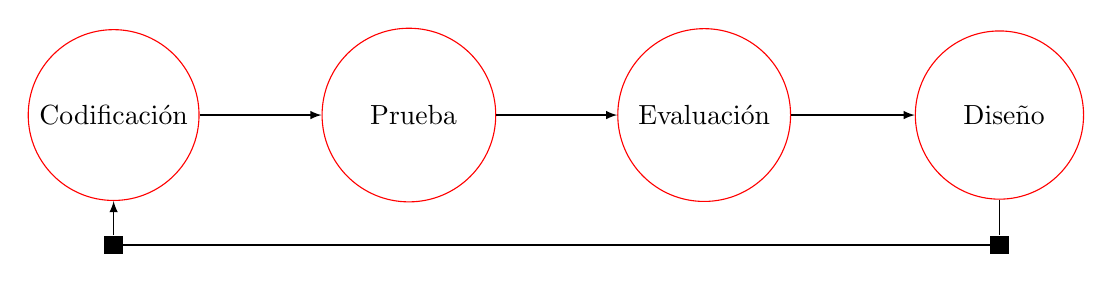
\begin{tikzpicture}[x=1.5cm, y=1.5cm]
	%\fill (-3.2,0) circle (0.1pt)node[anchor=east] {$20$};
	%\fill (3.2,0) circle (0.1pt)node[anchor=west] {$-20$};
    \node[circle,draw=red] (v1) at (-3.75,0) {Codificación};
    \node[circle,draw=red] (v2) at (-1.25,0) {\ \ \ \ Prueba\ \ \ \ };
    \node[circle,draw=red] (v3) at (1.25,0) {\ Evaluación\ \ };
    \node[circle,draw=red] (v4) at (3.75,0) {\ \ \ \ Diseño\ \ \ \ };
    \node[fill=black] (a1) at (-3.75,-1.1) {};
    \node[fill=black] (a2) at (3.75,-1.1) {};
    \draw[color=black, -latex]  (v1) edge (v2);
    \draw[color=black, -latex]  (v2) edge (v3);
    \draw[color=black, -latex]  (v3) edge (v4);
    %\draw[color=black]  (v4) edge (a2);
    %\draw[color=black]  (a2) edge (a1);
    \draw[color=black, -latex]  (a1) edge (v1);
    \draw (v4) -- (a2) -- (a1);
\end{tikzpicture}
\end{center}
\caption{Iteración de etapas en XP.}
\label{fig:fig1}
\end{figure}

En la figura \ref{fig:fig1} podemos observar un diagrama de las etapas estándar de XP. Si bien la primera etapa se corresponde normalmente con la codificación, en nuestro caso siempre lo ha sido el diseño. Así, para cada funcionalidad, se diseña la vista, se implementa la misma, a continuación se desarrolla y enlaza la lógica y por último se prueba. Se itera sobre estas etapas para cada vista y funcionalidad establecidas.

Se sigue así una planificación diseñada prácticamente para cada funcionalidad (planificación incremental) marcándose objetivos a muy corto plazo pero sin perder de vista el objetivo final: completar el programa y su correcto funcionamiento.

Para concluir, hemos tratado de hacer nuestro código lo más adaptable posible, no sólo por el tipo de proceso de desarrollo elegido, sino también para facilitar futuras implementaciones de nuevas funciones para el programa. Esto, sumado a todo lo contado en los anteriores párrafos, justifica que nuestro proceso de desarrollo se ajuste a XP y su correcta elección.

\section{\textit{Mutation Testing for Quantum Computing} (MTQC)}

MTQC son las siglas que dan nombre a nuestro programa. Su principal funcionalidad es la de aplicar pruebas de mutación en distintos lenguajes cuánticos, en nuestro caso \qsh\ y \textit{Qiskit}.

La secuencia de acciones de un usuario en poder de MTQC sería la de generar mutantes del programa deseado, verificar el resultado de los mutantes creados, ejecutar el programa original y los mutantes seleccionados dadas una serie de test y cotejar los resultados para encontrar test satisfactorios e indeseados.

Sobre estas cuatro fases hemos establecido toda nuestra planificación, análisis y diseño del proyecto y es así como vamos a explicar todo el proyecto, tomando estas etapas como estructura de cara al desarrollo.

\subsection{Principales funcionalidades}

Aunque el desarrollo dirigido por casos de uso no es propio de XP, nos inspiramos en ellos para determinar las principales funcionalidades del sistema que podemos identificarlas con las fases recientemente nombradas. Podríamos definir alguna otra adicional como el de elegir un lenguaje cuántico o el de reiniciar el programa, pero el grueso del contenido de MTQC lo recogen estas cuatro:

\begin{enumerate}
\item \textbf{Generación de mutantes}. Se trata de la primera acción que el usuario debe realizar. Consta de dos entradas consistentes en dos listas: una del directorio de los archivos de código sobre los que se quiere realizar mutación y otra de los operadores de mutación a aplicar. Arroja como salida una lista de mutantes vinculados al archivo original, el operador aplicado y la línea que sufrió la mutación. En caso de que la fabricación de un mutante arroje un error, se muestra un error por pantalla y se trata de generar el siguiente.

\item \textbf{Visualización de mutantes}. La precondición para que este caso de uso se pueda llevar a cabo es que previamente el usuario haya generado al menos un mutante. Toma como entrada una lista de mutantes con la que el usuario puede interactuar para así poder comparar el contenido de dicho mutante y el archivo original. El objetivo es que el usuario pueda tomar una decisión sobre si el mutante en cuestión es o no un candidato apto para ejecutar un test sobre él.

\item \textbf{Testeo de mutantes}. Se trata del caso de uso principal del programa por importancia, cantidad y calidad del código asociado al mismo. Es necesario verificar la precondición de haber generado al menos un mutante para realizar cualquier acción sobre el mismo. Enumeraremos las entradas.
	\begin{itemize}
	\item Un archivo de código del lenguaje cuántico elegido en ese momento.
	\item Una función contenida en el archivo anterior.
	\item Una lista de todos los mutantes deseados para ejecución generados a partir de dicho archivo.
	\item Un tipo de test a aplicar (determinista o probabilista).
	\item Un conjunto de test.
	\end{itemize}
	
La salida arrojará un conjunto de objetos que gestione los resultados arrojados tras la ejecución de los test y sobre la muerte o no de los mutantes.

\item \textbf{Visualización de los resultados de los test}. Por último, tenemos la opción de que el usuario vea los resultados que los test han arrojado al ser ejecutados sobre la función original y los mutantes, determinar cuántos de ellos han sido matados y la eficacias de dichos test. La precondición indispensable para llevar a cabo esta visualización es haber llevado a cabo las acciones mencionadas en el anterior caso de uso. Toma como entrada un conjunto de objetos que gestionan los resultados de los test y muestra la información correspondiente, previo tratamiento, por pantalla. En el caso de que el test realizado haya sido de tipo probabilista, tomará también como entrada un porcentaje de confianza.
\end{enumerate}

Esto se ha traducido en cuatro subsistemas bastante independientes; Sin embargo, en un principio, las funcionalidades 3 y 4 se pensaron para estar en un único subsistema y bajo una única vista. Esto cambió, principalmente, para no sobrecargar de información dicha vista y facilitar al usuario la lectura de los resultados dividiendo las funcionalidades en subsistemas distintos.

\subsection{Diseño}

Retomamos de nuevo las cuatro funcionalidades anteriores para esquematizar el programa. A la hora del diseño y desarrollo de MTQC se plantearon 4 subsistemas identificados cada uno a dichas funcionalidades.

Para implementar cada uno de los mismos se optó por por asignar a cada uno de ellos una pestaña visual independiente administradas bajo una misma vista conjunta. Esto se gestiona mediante el uso del patrón \textit{Modelo-Vista-Controlador} (MVC). Pese a no ser del todo necesario por poseer una única vista, se ha implementado el patrón \textit{Observador} en el que la vista actúa como observador y la lógica como sujeto. Este patrón se ha usado para facilitar la adición de futuras interfaces, gráficas o no, que se pudieran desarrollar sobre el proyecto.

En algunas partes del código ha sido utilizado el patrón \textit{Factoría}, por ejemplo, según el tipo de test escogido, este crea una instancia de una subclase concreta que gestiona los resultados arrojados por el test. Por otra parte, somos conscientes de que este mismo patrón es útil en combinación de \textit{Observador} y MVC para facilitar, precisamente, implementar otras interfaces. Sin embargo, decidimos no aplicarlo como tal para facilitar el código. Pese a ello, de ser necesario, su ejecución no presentaría cambios significativos en el código, sino más bien algunas adiciones en el mismo.

Detallaremos cada uno de estos subsistemas, pero antes vamos a exponer la jerarquía de paquetes que constituyen en programa y unas breves indicaciones sobre su contenido y funcionalidad.

\subsubsection{Estructuración del código por paquetes}

\begin{itemize}
\item \textbf{model}. Contiene toda la lógica del programa. Además de todos los paquetes que aparecen a continuación, contiene las clases que conforman el patrón \textit{Observador} (Observer y Observable) y la clase Model que gestiona el grueso de la lógica.
	\begin{itemize}
	\item \textbf{mutantoperator}. Recoge la clase abstracta MutantOperator que gestiona un operador de mutación.
		\begin{itemize}
		\item \textbf{qiskit} Contiene todas las implementaciones de operadores de mutación creados para \textit{Qiskit}.
		\item \textbf{qsharp} Contiene todas las implementaciones de operadores de mutación creados para \qsh.
		\end{itemize}		 
	\item \textbf{mutant}. Contiene la clase Mutant que gestiona un mutante tras su creación: ruta al archivo mutante, ruta al archivo original y línea de código que sufrió la mutación.
	\item \textbf{test}. Contiene la clase abstracta Test que gestiona las características del tipo de prueba a realizar, por ejemplo si es o no determinista. También contiene sus implementaciones.
	\item \textbf{run}. Recoge clases que gestionan las pruebas de mutación. Crea archivos ejecutables a partir de un mutante y una entrada de datos y los ejecuta.
	\item \textbf{files}. Contiene la clase TestFile que gestiona los archivos finales creados por las clases del paquete \textit{run}.
	\item \textbf{testresult}. Contiene la clases abstracta TestResult que gestiona los resultados de la ejecución de los test y también sus implementaciones, una por cada implementación de Test.
	\end{itemize}
\item \textbf{view}. Encargado de toda la vista del sistema.
	\begin{itemize}
	\item \textbf{mutantgeneartorview}. Contiene la vista correspondiente al primer subsistema.
	\item \textbf{mutantsviewer}. Contiene la vista correspondiente al segundo subsistema.
	\item \textbf{testcaserunnerview}. Contiene la vista correspondiente al tercer subsistema.
	\item \textbf{testresultview}. Contiene la vista correspondiente al cuarto subsistema.
	\item \textbf{tools}. Contiene algunas clases auxiliares utilizadas en la vista.
	\end{itemize}
\item \textbf{control}. Contiene la clase Control que actúa como controlador del patrón MVC.
\item \textbf{exception}. Recoge algunas excepciones del programa.
\item \textbf{main}. Recoge la clase Main que contiene el método que inicia la ejecución del programa.
\end{itemize}

Estamos en disposición de hablar de cada subsistema con detenimiento. Mencionaremos los paquetes involucrados en cada uno de ellos, detalles de implementación o la aparición de problemas relevantes y la solución adoptada para ellos.

\subsubsection{Subsistemas: Generador de mutantes}

\begin{figure}[htb]
\begin{center}
\includegraphics[scale=0.45]{images/vista1}
\end{center}
\caption{Vista del subsistema generador de mutantes.}
\label{fig:vista1}
\end{figure}

La generación de mutantes es el primer paso para realizar pruebas de mutación. En la figura \ref{fig:vista1} \ se contempla el aspecto de la vista asociada. La interfaz en su conjunto y cada una de las pestañas tiene un diseño simple, tratando de minimizar la cantidad de información para facilitar el uso y entendimiento del cliente.

Los componentes de esta vista se encuentran en el paquete view.mutantgeneratorview, aunque además hace uso de clases del paquete view.tools. En concreto, JTableCheck, que gestiona una tabla de  objectos de una determinada instancia junto a casillas verificadoras asociadas a booleanos y LogArea que imprime información para el usuario.

En cuanto a la lógica, los operadores se encuentran definidos todos ellos en el paquete model.mutantoperator, y los mutantes generados se gestionan para su uso en el resto del programa mediante la clase Mutant del paquete model.mutant.

La vista ofrece al usuario una lista de archivos en un determinado directorio que puede ser cambiado por el usuario. También aparece una lista de operadores de mutación acorde con en lenguaje cuántico seleccionado en ese momento. Tras la selección de los archivos y operadores se procede a llamar al controlador para que ordene a la lógica la creación de los mutantes.

Para la generación de mutantes se ha implementado la técnica del programador hábil, sólo se aplica una mutación a cada archivo generado. El proceso que sigue la lógica es sencillo, un operador contiene una secuencia de caracteres a ser buscada y otra con la que es reemplazada. Así, por cada archivo y operador, se generan tantos mutantes como veces se encontró dicha cadena. Todas estas acciones se realizan desde las clase Model.

De haber algún reto en esta fase del desarrollo, se trataría del hecho de establecer cuando hemos encontrado una cadena de caracteres coincidente con la mutación que queremos incurrir. En el caso de \textit{Qiskit} es sencillo, pues todas las instrucciones cuánticas son métodos que son llamados mediante un objeto perteneciente a la clase QuantumCircuit. Así, todas las instrucciones son del siguiente estilo

\begin{center}
objeto.instrucción(...)
\end{center}

y por tanto podemos buscar la cadena \textbf{.instrucción(} y sustituirla por \textbf{.mutación(} donde las palabras instrucción y mutación representan la conversión requerida. En el caso de \qsh\ no es tan sencillo, ya que las instrucciones tienen el aspecto de

\begin{center}
instrucción(...)
\end{center}

así que no basta con sustituir \textbf{instrucción(} por \textbf{mutación(}. Supongamos que queremos realizar mutantes cambiando el operador de la puerta de \textit{Hadamard}, representado por la instrucción H(...), por la puerta X, si en el proceso encontrásemos un método (por raro que fuera) acabado en H, por ejemplo applyH(...), estaríamos generando un mutante en el que esa instrucción sería cambiada por applyX(..) que no es el efecto que deseamos. La solución a esto es comprobar el carácter anterior y verificar que se trata de un salto de línea, un espacio o una tabulación.

Otro problema similar se aplica a los operadores de mutación aplicados a constantes en \qsh como \textbf{One} y \textbf{Zero}. La solución es, de nuevo, la comentada en el párrafo anterior pero aplicando dicha comprobación también al carácter posterior.

\subsubsection{Subsistemas: Visualizador de mutantes}

El segundo subsistema es el más simple de los cuatro. Se trata de una vista sencilla (figura \ref{fig:vista2}) que muestra la lista de mutantes generados y dos áreas de de texto, que actúan como \textit{display} de los ficheros original y mutante. Si no se han generado mutantes previamente, la lista aparecerá vacía.

\begin{figure}[htb]
\begin{center}
\includegraphics[scale=0.45]{images/vista2}
\end{center}
\caption{Vista del subsistema visualizador de mutantes.}
\label{fig:vista2}
\end{figure}

La lista de mutantes se gestiona mediante la clase JMutantList en el paquete view.tools. El resto de componentes se gestionan desde las clases FileArea y MutantsViewer del paquete view.mutantsviewer. Además, la lista antes mencionada contiene, no sólo el identificador del mutante, sino la instancia al completo.

El funcionamiento es sencillo, el usuario debe pinchar sobre el mutante que quiera ser observado y la vista puede obtener de dicho mutante las rutas a los archivos original y mutado sin necesidad de hacer llamada al controlador y, por tanto, tampoco al modelo. Tal vez en este caso no se esté siguiendo las directrices del patrón MVC como es debido, pero por su simplicidad optamos por este camino.

\subsubsection{Subsistemas: Pruebas de mutación y creación de test}

Es sin duda el componente más complejo del programa. En él intervienen gran parte de la lógica realizada para el proyecto. La funcionalidad se resume en ejecutar una elección de mutantes con unos casos de prueba determinados para decretar qué porcentaje de ellos ha sido matado y la eficacia de dichas pruebas.

\begin{figure}[htb]
\begin{center}
\includegraphics[scale=0.45]{images/vista3}
\end{center}
\caption{Vista del subsistema pruebas de mutación y creación de test.}
\label{fig:vista3}
\end{figure}

En la figura \ref{fig:vista3} tenemos la vista que constituye el subsistema cuyos componentes se engloban dentro del paquete view.testcaserunnerview y, además, hace uso de las clases del paquete view.tool TabbedTextArea, que gestiona las entradas para los casos de prueba que el usuario puede introducir mediante un sistema de pestañas; JTableCheck, tabla que gestiona la selección de mutantes; TextField, un simple campo de texto y LogArea, que imprime información de la ejecución del programa al usuario.

Aunque el usuario podía en el primer subsistema seleccionar más de un archivo para aplicar mutaciones sobre él, para realizar las pruebas de mutación debemos hacerlo, en este caso, de manera individual. Además, los archivos que MTQC genera para ejecutar todas las pruebas se almacenan en una carpeta auxiliar; Por tanto, el programa a probar no podrá usar archivos o librerías que no estén en el directorio por defecto del lenguaje correspondiente. Para solucionar esto, el usuario puede incluir la ruta a los archivos necesarios en el propio programa. Por ejemplo en \textit{Python} puede hacerse con

\begin{figure}[htb]
\begin{lstlisting}[language=Python]
import sys
sys.path.insert(0, "path_to_your_package")
\end{lstlisting}
\caption{Código para añadir una nueva ruta donde \textit{Python} buscará módulos.}
\label{fig:code1}
\end{figure}

aunque, en general, los programas cuánticos rara vez alcanzan una extensión suficiente para ser modulados en varios archivos y no debe ser un problema en la mayoría de casos.

Así, la primera decisión que ha de tomar el usuario es la de elegir el archivo deseado. En la vista se muestran los correspondientes a la ruta seleccionada en el primer subsistema. Tras la elección, se llama al controlador para que la lógica realice dos tareas. La primera es obtener todos los mutantes generados a partir del archivo seleccionado; la segunda es devolver todas las funciones encontradas en el archivo.

El usuario debe ahora realizar el resto de la configuración: Elegir los mutantes a ejecutar, la función de llamada, el tiempo límite para la ejecución de cada prueba (para evitar ejecuciones infinitas debido a que nos hayamos quedado en un bucle a causa de la mutación), el tipo de test, elegir el número de ejecuciones si este último es probabilista y , por último, las entradas o test.

En cuanto al tipo de test, está implementado uno determinista que hemos denominado \textbf{\textit{QStateTest}} y otro probabilista, \textbf{\textit{ProbabilisticTest}}. El primero compara las probabilidades arrojadas por los estados finales del sistema cuántico. Supongamos que una función sobre un sistema cuántico de un qubit devuelve $\frac{1}{\sqrt{2}}\ket{0}+\frac{1}{\sqrt{2}}\ket{1}$ mientras que el mutante devuelve $\frac{1}{\sqrt{2}}\ket{0}-\frac{1}{\sqrt{2}}\ket{1}$, este test evalúa las probabilidades de cada estado, que en ambos casos son de $\frac{1}{2}$ para $\ket0$ y un $\frac{1}{2}$ para $\ket1$. Por tanto no se mataría al mutante pese a que los estados cuánticos no son idénticos.

Sobra decir que este test solo es posible si se ejecuta sobre un simulador en un computador clásico. Para su implementación, en el caso de \qsh\ hemos hecho uso de la instrucción \textbf{DumpMachine()} que imprime en un fichero o pantalla el estado cuántico en ese momento, mientras que el simulador \textbf{StatevectorSimulator} de \textit{Qiskit} permite de igual modo acceder a dicha información.

El segundo tipo de test, \textit{ProbabilisticTest}, compara la salida final de la función que, generalmente, será la medición de uno o más qubits. Por tanto, esta salida puede ser probabilista y su ejecución puede ser realizada en repetidas ocasiones con el fin de conseguir una certeza estadística sobre la muerte o no del mutante. Dicho test puede ser aplicado en computadoras cuánticas usando \textit{Qiskit}, basta con seleccionar una máquina de \textit{IBM} disponible para la ejecución escribiendo el código correspondiente en la entrada. Sin embargo, hay que tener en cuenta que la disponibilidad de estas computadoras es muy limitada y las ejecuciones mensuales también lo son, así que podría demorar bastante tiempo.

Como vimos en el capítulo anterior, la inicialización del estado cuántico deseado supone un problema añadido respecto de la computación clásica. El usuario debe darnos una secuencia de puertas para conseguir el estado de entrada deseado. En el caso de \textit{Qiskit} existe una función del circuito cuántico (QuantumCircuit), \textbf{initialize()}, que permite inicializar el circuito en el estado deseado, siempre que el simulador utilizado sea StatevectorSimulator.

\begin{figure}[htb]
\begin{lstlisting}[language=Python]
from qiskit import *
import numpy as np

qr = QuantumRegister(3)
qc = QuantumCircuit(qr)
init = [complex(0, 1/np.sqrt(2)), 0, 0, complex(1/np.sqrt(2), 0), 0, 0, 0, 0]
qc.initialize(init, qr)
\end{lstlisting}
\caption{Inicialización de un circuito cuántico mediante un vector complejo en \textit{Qiskit}.}
\label{fig:code2}
\end{figure}

El código anterior inicializa el circuito cuántico de 3 qubits en el estado $\frac{i}{\sqrt{2}}\ket{000}+\frac{1}{\sqrt{2}}\ket{011}$. Nótese que el vector dado como ejemplo tiene norma uno; en otro caso la ejecución nos arrojaría un error.

En cualquier caso, la preparación de la entrada requiere un tratamiento previo. Para tratar esta entrada hemos facilitado dos métodos. El primero es mediante la carga de un archivo de texto en el que cada caso es separado por una línea con la secuencia de caracteres \textbf{***} y cada caso tiene que tener la estructura del segundo método que mencionamos a continuación. El segundo es un sistema de pestaña. Por defecto aparece una pestaña con un ejemplo estructural a seguir y en el caso de de añadir una nueva, aparece con una copia del contenido de la seleccionada previamente. El código dado por defecto para \textit{Qiskit} está reflejado en la figura \ref{fig:code3}.

\begin{figure}[htb]
\begin{lstlisting}[language=Python]
def init ():
	cr = ClassicalRegister(1)
	qr = QuantumRegister(1)
	qc = QuantumCircuit(qr, cr)

	# Initialize with desired quantum gates or QuantumCircuit.initialize() method

	# Call your method

	ex = execute(qc, backend = Aer.get_backend('statevector_simulator'))

	# Add any operations if needed
	
	return next(iter(ex.result().get_counts())) # Change desired return
	#return pow(abs(ex.result().get_statevector()), 2) # If probabilistic test chosen
\end{lstlisting}
\caption{Código dado por defecto en MTQC para inicializar un caso de prueba en \textit{Qiskit}.}
\label{fig:code3}
\end{figure}

Según lo deseado, podemos modificar el número de registro clásicos (\textbf{ClassicalRegister}) y cuánticos (\textbf{QuantumRegister}), añadir la inicialización deseada en cada caso y debemos llamar al método elegido. Por último, habrá que habrá que comentar uno de los dos \textit{return} en función al tipo de test elegido según se indica o incluso puede ser cambiado para devolver otro tipo de datos si se desea. Es importante recalcar que \textit{Qiskit} construye un circuito con el uso de métodos de aplicación de puertas, pero realmente ese circuito no se ejecuta hasta que no se llama a la instrución \textbf{execute(...)}. Si esta función es llamada durante el método que será probado, basta con comentar o borrar la línea de código correspondiente de la figura \ref{fig:code3}.

En cualquier caso, debemos mantener la tabulación establecida y no cambiar el nombre del método definido en la primera línea, pues es llamado para poder ser inicializada la entrada. Si es opta por la introducción vía archivo, este método tiene que estar definido para cada caso de igual modo.

\begin{figure}[htb]
\begin{lstlisting}[language=c++]
//Select desired Qubit number to be used
using (register = Qubit[2]) {

	//Inicialize variables and Qubits
	let count = 1;
	let initial = Zero;

	//Call method and save output
	let(output) =  method(...);

	//If probabilistic test chosen.
	//DumpMachine("temp.txt");

	//Reset all qubits to Zero state
	ResetAll(register);

	//Return output
	return output;
}
\end{lstlisting}
\caption{Código dado por defecto en MTQC para inicializar un caso de prueba en \qsh.}
\label{fig:code4}
\end{figure}

Las mismas indicaciones tenemos para \qsh\ (figura \ref{fig:code4}), debemos mantener la estructura general y modificar lo necesario siguiendo las indicaciones, ya haya sido elegido el método de entrada mediante el uso de la vista de pestañas o mediante la carga de archivo.

Tenemos así todo listo para proceder: archivo, método, mutantes, tipo de test y casos de prueba, entre otros. Todos estos datos se gestionan con las clases mencionadas anteriormente para cada uno de ellos. El usuario está listo para ejecutar los test, así, la vista llama al controlador que preprocesa los datos antes de mandárselos a la lógica. El primer objetivo es preparar nuevos archivos que añadan las entradas establecidas a los archivos a ejecutar: mutantes y original. Dichos archivos son creados por las clases del paquete model.run y gestionadas por la clase TestFile del paquete model.files.

El siguiente paso es generar un archivo principal en \textit{Python} que será ejecutado mediante una llamada al sistema (por tanto el usuario debe tener agregado \textit{Python} en su \textit{path}) y que llamará a todos los archivos generados en el paso anterior para obtener las salidas arrojadas por los test.

Tras ser ejecutados, MTQC recoge las salidas resultantes de la ejecución asignándolas al archivo original o mutante y a uno de los test según corresponda. Esta gestión de datos se realiza mediante una de las clases del paquete model.testresult según el tipo de test elegido.

Para acabar, todos los archivos generados durante esta fase son borrados y se manda una actualización de los resultados obtenidos al último subsistema que veremos a continuación.

\subsubsection{Subsistemas: Visualizador de resultados}

En último lugar tenemos el subsistema dedicado a visualizar los resultados. La vista (figura \ref{fig:vista4}) es un sencillo sistema de pestañas, una para cada test, que contiene una tabla donde se comparan los resultados y se indica qué mutantes han muerto y cuáles no.

Los componentes de la vista se encuentran íntegramente en el paquete view.testresultview a excepción de la clase ResultTable, que gestiona cada tabla, del paquete view.tools. Como hemos mencionado, los resultados que se muestran en esta vista se actualizan automáticamente al final de la ejecución del subsistema anterior.

\begin{figure}[htb]
\begin{center}
\includegraphics[scale=0.45]{images/vista4}
\end{center}
\caption{Vista del subsistema visualizador de resultados.}
\label{fig:vista4}
\end{figure}

Además, el usuario puede modificar la confianza utilizada para matar a un mutante en un test probabilístico, veamos como funciona. Supongamos que tenemos un total de $n$ estados posibles ($\ket0,...,\ket{n-1}$) en cierto sistema cuántico y hemos ejecutado $k$ veces tanto el archivo original como el mutante. Definimos las probabilidades de medición del estado cuántico $\ket i$ para el archivo original como

\begin{equation}
p_{\ket i,o}=\dfrac{f_{\ket i,o}}{k}
\end{equation}

donde $f_{\ket i,o}$ denota el número de veces que la salida del programa original fue el estado $\ket i$. Análogamente, para cierto archivo mutante $m$ definimos las probabilidades de medición del estado cuántico $\ket i$ como

\begin{equation}
p_{\ket i,m}=\dfrac{f_{\ket i,m}}{k}
\end{equation}

donde $f_{\ket i,m}$ denota el número de veces que la salida del mutante $m$ fue el estado $\ket i$. Así un mutante $m$ muere si se verifica

\begin{equation}
\max \{|p_{\ket i,o}-p_{\ket i,m}|:0\leq i\leq n - 1\}> c
\end{equation}

donde $c$ denota el parámetro de confianza que puede ser manipulado por el cliente. Obviamente el máximo del conjunto anterior está comprendido entre 0 y 1 por estarlo las probabilidades definidas anteriormente. El parámetro de confianza en MTQC por defecto es del 1\%, pero puede modificarse al porcentaje deseado. Tras esto, se contactará con la clase Model de la lógica que solicitará a cada instancia de la clase TestResult que recalcule la muerte o no del mutante en función del nuevo valor indicado y comunicará a la vista los resultados.

\section{Implementaciones futuras}

Para finalizar este capítulo queremos aportar algunas ideas con las que se puede dar continuidad a este proyecto. Algunas de estas funcionalidades fueron planificadas al principio del proyecto para ser descartadas más adelante y otras surgen durante la implementación de MTQC.

\begin{itemize}
\item Implementación de \textit{weak mutation testing}. Se trataría de un test determinista a realizar sobre simulador que verificara las condiciones de la definición \ref{def:def24}.

\item Facilitar el uso de otros archivos y librerías externas. Como mencionamos antes, el usuario debe realizar una adición de código para encontrar la ruta a estos archivos y seria conveniente que esto no fuera necesario.

\item Añadir algún lenguaje adicional como \textbf{OpenQASM}.

\item Permitir que el usuario pueda añadir nuevos operadores de mutación desde la ejecución del programa y que estos puedan ser guardados para futuras pruebas de mutación.

\item Permitir guardar el proceso de una ejecución, como mutantes y otras configuraciones, para que la tarea pueda ser retomada en otra ejecución.
\end{itemize}

% Ejemplos y conclusiones
%\chapter{Ejemplos y conclusiones}

Vamos a dar uso a MTQC. Implementaremos el algoritmo de \textit{Deutsch-Jozsa} [\cite{deutsch1992rapid}] en los lenguajes \textit{Qiskit} y \qsh\ y aplicaremos pruebas de mutación sombre ambos códigos. Antes veremos que problema plantea dicho algoritmo.

Por último se discuten algunas ideas propicias para la mejora y continuidad del proyecto.

\section{Pruebas de mutación sobre Deutsch-Jozsa}

Sea $\function{f}{\{0,1\}^n}{\{0,1\}}$ una función binaria que bien puede ser constante ($f(x) = 0$ o $f(x) = 1$ para todo $x\in\{0,1\}^n$) o bien es balanceada (la salida es 0 para la mitad de entradas y 1 para la otra mitad). Desde el punto de vista clásico, en el caso peor hay que verificar $2^{n-1}+1$ entradas para resolver el problema. El algoritmo cuántico de \textit{Deutsch-Jozsa} lo resuelve en una sola iteración.

\subsection{Algoritmo Deutch-Jozsa}

Previamente a mostrar el código de nuestro ejemplo particular, analicemos en detalle cada paso del que consta el algoritmo de Jozsa.

En primer lugar, si nuestra función $f$ toma valores en $\{0,1\}^n$, debemos crear un circuito con $n + 1$ qubits. Todos los qubits deberan tomar el estado $\ket{0}$ menos el último de ellos, que utilizaremos como auxiliar e inicializamos al estado $\ket{1}$. De esta forma nuestro sistema se encuentra en un primer estado dado por:
\begin{equation}
\ket{\phi_0} = \ket{0\overset{n}{\cdots}01}
\end{equation}

A continuación, aplicamos una puerta Hadamard a cada qubit, obteniendo de esta forma el siguiente estado:
\begin{equation}
\ket{\phi_1} = \dfrac{1}{\sqrt{2^{n+1}}} \sum\limits_{i=0}^{2^n - 1} \ket{i}(\ket0-\ket1) \textrm{, donde $i$ se corresponde con su representación binaria.}
\end{equation}

Posteriormente, hay que aplicar el operador $U_f$ tal y como fue definido en \ref{uf}. Si denotamos por $x$ a los $n$ qubits de entrada y por $y$ al qubit auxiliar se tiene:
\begin{equation}
U_f\colon \begin{matrix}x&\longrightarrow& x\\ \y&\longrightarrow& y\oplus f(x)\end{matrix}
\end{equation}

El diseño de esta $U_f$ puede ser muy complejo, dependiendo de cómo sea la función $f$. En nuestro ejemplo hemos escogido una función que facilita la creación del operador $U_f$.

Tras aplicar el operador $U_f$, se obtiene un tercer estado dado por:
\begin{equation}
\ket{\phi_2} = \dfrac{1}{\sqrt{2^{n+1}}} \sum\limits_{i=0}^{2^n - 1} \ket{i}(\ket{f(i)}-\ket{1\oplus f(i)}) 
\end{equation}

Ahora, como $f(i)$ sólo puede tomar valores binarios, podemos simplificar la expresión anterior:
\begin{equation}
\ket{\phi_2} = \dfrac{1}{\sqrt{2^{n+1}}} \sum\limits_{i=0}^{2^n - 1} (-1)^{f(i)}\ket{i}(\ket0-\ket1) 
\label{phi2}
\end{equation}


A partir de este punto, el estado del último qubit $\dfrac{1}{\sqrt{2}}(\ket0-\ket1)$ puede ser ignorado, pues no será relevante para el resto de cálculos.

A continuación, debemos aplicar una puerta Hadamard a cada uno de los $n$ qubits restantes. Previamente a realizar dicha operación, vamos a ver cómo una representación matemática de la aplicación simultanea de puertas Hadamard que facilita la comprensión de la parte final del algoritmo.

Cuando contamos con un sólo qubit, una puerta Hadamard sabemos que viene dada por: \[\gatetwo{H}{\dfrac{1}{\sqrt{2}}(\ket0+\ket1)}{\dfrac{1}{\sqrt{2}}(\ket0-\ket1)}\]

Por tanto, podemos escribir el caso general, donde $x=0$ o $x=1$ como:
\begin{equation}
H\ket{x} = \tfrac{1}{\sqrt{2}}\sum\limits_{z\in\{0,1\}} (-1)^{x\cdot z}\ket{z} \textrm{, donde $x\cdot z$ denota el producto escalar bit a bit, módulo 2.}
\end{equation}

Veamos ahora el caso con 2 qubits a los que aplicamos una puerta Hadamard a cada uno:
\begin{equation}
\begin{split}
H^{\otimes 2}\ket{x_1,x_2} & = H\ket{x_1} \otimes H\ket{x_2} \\
& = \tfrac{1}{\sqrt{2}}\sum\limits_{z_1\in\{0,1\}} (-1)^{x_1\cdot z_1}\ket{z_1} \otimes \tfrac{1}{\sqrt{2}}\sum\limits_{z_2\in\{0,1\}} (-1)^{x_2\cdot z_2}\ket{z_1} \\
& = \tfrac{1}{\sqrt{2^2}}\sum\limits_{z_1,z_2\in\{0,1\}} (-1)^{x_1\cdot z_1+x_2\cdot z_2}\ket{z_1,z_2}
\end{split}
\end{equation}

De esta misma forma, podemos representar la aplicación de puertas Hadamard a $n$ qubits como:
\begin{equation}
\begin{split}
H^{\otimes n}\ket{x_1,\cdots,x_n} & = \tfrac{1}{\sqrt{2^n}}\sum\limits_{z_1,\cdots,z_n\in\{0,1\}} (-1)^{x_1\cdot z_1+\cdots+x_n\cdot z_n}\ket{z_1,\cdots,z_n}
\end{split}
\end{equation}

Si retomamos ahora la notación para el sumatorio utilizada a lo largo de la demostración, podemos expresar el resultado anterior como:
\begin{equation}
\begin{split}
H^{\otimes n}\ket{x_1,\cdots,x_n} & = \tfrac{1}{\sqrt{2^n}}\sum\limits_{z=0}^{2^n-1} (-1)^{x\cdot z}\ket{z}
\end{split}
\end{equation}

Por tanto, partiendo de la expresión \ref{phi2}, si aplicamos una puerta Hadamard a los $n$ primeros qubits (recordemos que el estado del último qubit ya no era relevante),
se obtiene un nuevo estado $\phi_3$ dado por:

\begin{equation}
\begin{split}
\ket{\phi_3} & = \dfrac{1}{\sqrt{2^{n}}} \sum\limits_{i=0}^{2^n - 1} (-1)^{f(i)}\left[\dfrac{1}{\sqrt{2^{n}}}\sum\limits_{j=0}^{2^n - 1}(-1)^{i\cdot j}\ket{j}\right] \\
& = \dfrac{1}{2^n}\sum\limits_{j=0}^{2^n - 1}\left[\sum\limits_{i=0}^{2^n - 1}(-1)^{f(i)}(-1)^{i\cdot j}\right]\ket{j}
\end{split}
\label{phi3}
\end{equation}

Una vez que hayamos obtenido este estado, vamos a estudiar cual es la probabilidad de obtener el estado $\ket{0\overset{n}{\cdots}0}$ al medir los $n$ primeros qubits.

En virtud de (\ref{phi3}), el cuadrado de la amplitud del estado $\ket{0\overset{n}{\cdots}0}$ viene dada por:

\begin{equation}
\begin{split}
& \left|\dfrac{1}{2^n}\sum\limits_{i=0}^{2^n - 1}(-1)^{f(i)}(-1)^{i\cdot j}\right|^2 \\ 
= &\left|\dfrac{1}{2^n}\sum\limits_{i=0}^{2^n - 1}(-1)^{f(i)}\right|^2 \textrm{, ya que j = $0\overset{n}{\cdots}0$}
\end{split}
\end{equation}

Por tanto, si la \emph{función $f$ es balanceada}, la mitad de los términos $(-1)^{f(i)}$ evaluaran a $1$, mientras que la otra mitad a $-1$, otorgando por tanto \emph{probabilidad 0} de obtener el estado 
$\ket{0\overset{n}{\cdots}0}$.

Si por el contrario la \emph{función $f$ es constante}, entonces todos los términos $(-1)^{f(i)}$ tendrán el mismo signo, no cancelándose entre ellos, y por tanto obteniendo \emph{probabilidad 1} de medir el estado $\ket{0\overset{n}{\cdots}0}$.

De esta forma, se puede discernir de manera completamente determinista si la función $f$ es constante o balanceada. En la figura \ref{fig:fig61} podemos ver el circuito que resume todo lo contado anteriormente.

\begin{figure}[!htb]
\[\Qcircuit @C=1em @R=.7em {
\lstick{\ket{0}} & \qw & \gate{H} & \qw &\multigate{4}{U_f}&\qw& \gate{H} & \qw & \meter & \qw \\
\lstick{\ket{0}} & \qw & \gate{H} & \qw & \ghost{U_f}      &\qw& \gate{H} & \qw & \meter & \qw \\
\lstick{\ket{0}} & \qw & \gate{H} & \qw & \ghost{U_f}      &\qw& \gate{H} & \qw & \meter & \qw \\
\lstick{\ket{0}} & \qw & \gate{H} & \qw & \ghost{U_f}      &\qw& \gate{H} & \qw & \meter & \qw \\
\lstick{\ket{1}} & \qw & \gate{H} & \qw & \ghost{U_f}      &\qw& \qw      & \qw & \qw    & \qw}\]
\caption{Circuito de una implementación de Deutsch-Jozsa.}
\label{fig:fig61}
\end{figure}

\subsection{Deutsch-Jozsa en MTQC}

Una vez que hemos visto cuales son los pasos a aplicar para ejecutar el algoritmo de Deutsch-Jozsa, se procede a exponer el código de dicho algoritmo para los lenguajes $\qsh$ y \textit{Qiskit} además de las funciones $f$ utilizadas. Empecemos por estas últimas.

Emplearemos 3 funciones $\{0,1\}^4\longrightarrow\{0,1\}$ que vienen definidas por:
\begin{itemize}
\item $f_1(x_1,x_2,x_3,x_4)=\left\{\begin{matrix}1 \mathrm{\ si\ } x_1=1\\0 \mathrm{\ si\ } x_1=0\end{matrix}\right.$, por lo que se trata de una función balanceada.

\item $f_2(x_1,x_2,x_3,x_4)=0$, por lo que se trata de una función constante.

\item $f_3(x_1,x_2,x_3,x_4)=1$, por lo que se trata de una función constante.
\end{itemize}

\begin{figure}[!htb]
\begin{lstlisting}[language=Python]
def deutschjozsa (qc, qr, cr, uf):
    if len(qr) != 5:
        print("El numero de qubits debe ser 5.")
        return
    
    # Negacion  del ultimo qubit
    qc.x(qr[-1])
    
    # Aplicacion de una puerta de Hadamard a cada qubit
    for r in qr:
        qc.h(r)
        
    # Aplicamos U_f
    uf(qc, qr)
        
    # Aplicacion de una puerta de Hadamard a cada qubit de entrada
    for r in qr[:-1]:
        qc.h(r)
            
    qc.measure(qr[:-1], cr)

def uf_1 (qc, qr):
    # f(x_1,x_2,x_3,x_4) = 1 si x_1 vale 1, 0 en otro caso. Balanceada
    # U_f cnot, como control el primer cubit, X aplicada a qubit de salida
    qc.cx(qr[0], qr[-1])
    
def uf_2 (qc, qr):
    # f(x_1,x_2,x_3,x_4) = 0. Constante
    # U_f Identidad qubit de salida
    qc.iden(qr[-1])
    
def uf_3 (qc, qr):
    # f(x_1,x_2,x_3,x_4) = 1. Constante
    # U_f not en qubit de salida
    qc.x(qr[-1])
\end{lstlisting}
\caption{Código en \textit{Qiskit} de una implementación de Deutsch-Jozsa.}
\label{fig:code62}
\end{figure}

Las $U_f$ respectivas son fáciles de implementar. En el primer caso basta con aplicar una puerta CNOT empleando como controlador el qubit correspondiente al bit $x_1$ y como qubit receptor el de salida. En el caso de $U_{f_2}$ no hay que realizar ninguna operación, aunque pondremos simbólicamente la puerta identidad aplicada al qubit de salida. Por último, $U_{f_3}$ viene determinada por una puerta $X$ aplicada al qubit de salida.

En la figura \ref{fig:code62} podemos ver el código en \textit{Qiskit} de la implementación del algoritmo de \textit{Deutsch-Jozsa} para un sistema de 5 qubits y cada una de las funciones $U_f$ expresadas anteriormente, mientras que en la figura \ref{fig:code63} encontramos el mismo algoritmo en \qsh.

En primer lugar, tratamos de la generación de mutantes. Utilizando MTQC sobre los ficheros que contienen los algoritmos (que no incluyen las funciones $U_f$) obtenemos un total de 9 mutantes en le caso de \textit{Qiksit}, mientras que en \qsh\ obtenemos 10. Esencialmente, son los mismos 9 mutantes en uno y otro lenguaje, sólo que \qsh tiene uno adicional que cambia la constante \textit{One} por \textit{Zero}. En cuanto a los comunes son distintas mutaciones de las puertas $H$ y $X$ a otras puertas unitarias.

Ya tenemos todo listo para la ejecución de nuestro algoritmo. En este caso, el valor de los qubits de entrada debe ser $\ket{00000}$; carece de sentido introducir valores distintos, pues el correcto funcionamiento del algoritmo depende de que se verifique dicho estado al comienzo de la ejecución.

Sí podemos, sin embargo, utilizar cada una de las $U_f$ definidas como parámetro de entrada. En el caso de \textit{Qiskit}, al estar escrito sobre \textit{Python}, permite la definición de una función de manera local y utilizarla como argumento de un método sin necesidad de especificar el tipado (pues \textit{Python} carece del mismo). Por otro lado, \qsh\ requiere la definición de dicho tipado y, además, no permite la definición de funciones de manera local, por lo que debemos hacerlo de manera global.

Vamos a ejecutar ambos tipos de pruebas de mutación presentes en MTQC sobre 3 test, uno por cada $U_f$ definida. Comencemos con \textit{ProbabilisticTest}. Para ello se ha tomado la decisión de ejecutar cada mutante con cada test un total de 1000 iteraciones. Nótese que pese al determinismo de este algoritmo, los mutantes generados pueden no serlo. Hemos adecuado la salida para que sea una cadena de caracteres que retorne ``balanceada'' o ``constante'' según corresponda.

Analicemos los resultados obtenidos para este tipo de test en cada uno de los lenguajes. Cabe mencionar que el parámetro de confianza utilizado en ambos casos ha sido del $1\%$.

En el caso de la ejecución del primer test, el resultado para ambos lenguajes es muy similar. En Qiskit, se han matado 8 de los 9 mutantes generados (\textit{Mutant Score} de $88.9\%$), mientras que en \qsh\ el mutante adicional sobrevive, luego se obtiene un \textit{Mutant Score} de $80\%$. Es interesante analizar el mutante común superviviente, y lo haremos al final de esta sección, pues adelantamos que sobrevive a los 3 test realizados.

\begin{figure}[H]
\begin{lstlisting}[language=c++]
operation DeutschJozsa(register : Qubit[], U_f : (Qubit[] => Unit)) : String {
	let nQubits = Length(register);
    if (nQubits != 5) {
   		return "El numero de Qubits debe ser 5 ";
    }
    else {
    	//Negacion del ultimo Qubit (salida)
        X(register[nQubits - 1]); 
        //Poner cada qubit en superposicion
        for(q in register) {
        	H(q);
        }         
        //Aplicamos la Uf
        U_f(register);
        //Aplicamos una puerta Hadamard a cada Qubit de entrada
        for(i in 0..nQubits - 2) {
        	H(register[i]);
        }        
        //La funcion sera constante si medimos el estado 0000. Balanceada en otro caso.
        mutable allZeros = true;
        for(i in 0..nQubits - 2) {
           	if(M(register[i]) == One){
            	set allZeros = false;
            }
        } 
        if (allZeros){
        	return "Constante";
        } else {
        	return "Balanceada";
        }
	}
}
operation uf(register : Qubit[]) : Unit{
		//f(x_1,x_2,x_3,x_4) = 1 si x_1 vale 1, 0 en otro caso. Balanceada
		CNOT(register[0], register[Length(register) - 1]);
}

operation uf2(register : Qubit[]) : Unit{
		//f(x_1,x_2,x_3,x_4) = 1. Constante
		I(register[Length(register) - 1]);
}

operation uf3(register : Qubit[]) : Unit { 
		//f(x_1,x_2,x_3,x_4) = 0. Constante  
		X(register[Length(register) - 1]);
}
\end{lstlisting}
\caption{Código en \qsh\ de una implementación de Deutsch-Jozsa.}
\label{fig:code63}
\end{figure}

Para el segundo test, de nuevo se obtienen resultados semejantes entre ambos lenguajes. Qiskit consigue matar 6 de 9 mutantes (\textit{Mutant Score} de $66.7\%$), y \qsh\ elimina a los mismos mutantes y al adicional, obteniendo un \textit{Mutant Score} de $70\%$. 

Por último, los resultados generados para el tercer test es análogo para Qiskit y \qsh. En ambos, los resultados son idénticos (salvo pequeñas variaciones en los porcentajes de las salidas, que podrían aproximarse mediante la ejecución de un mayor número de iteraciones) a los obtenidos en el segundo test.

En total, mediante estos tres test, se eliminan todos los mutantes menos uno de ellos. Este mutante es el obtenido mediante la sustitución de la puerta X, que niega el qubit de salida, por la puerta Y. Esto se debe a que al aplicar una puerta X o Y al estado $\ket{0}$ se obtiene el mismo estado $\ket{1}$ módulo un cambio de fase global, por lo que el comportamiento cuántico de ambos estados es el mismo. De esta forma, se obtiene un mutante equivalente que sobrevivirá independientemente del test. 

En conclusión podemos determinar que el Test1 es el más adecuado, no solamente por tener un \textit{Mutant Score} más elevado, sino porque Test2 y Test3 se identifican con una $U_f$ que representa una función constante. Independientemente de la dimensión del espacio de entrada, sólo existen dos funciones constantes: la función constante cero y la función constante uno, cuya $U_f$ asociada se construye mediante una única puerta I o X, respectivamente, aplicada exclusivamente al qubit de salida, que es el único que no es relevante a la hora de medir. Esto implica que todas las mutaciones realizadas sobre los operadores que afecten a dicho qubit (en nuestro caso la puerta X), no sean detectadas en el caso de que función sea constante. Es por esto que el Test1, al representar una función balanceada, es propenso a eliminar este tipo de mutantes.

Por último, analicemos los resultados obtenidos a la hora de ejecutar el \textit{QStateTest}. Debido a la naturaleza determinista de este algoritmo, este tipo de test no es el más indicado. Para una mejor adaptación, se ha considerado adecuado eliminar las lineas de código referentes a la medición, pues esta altera de manera no determinista el estado interno del programa. Es por esto que ahora disponemos 9 mutantes para cada lenguaje, pues el mutante adicional que teníamos previamente para \qsh\ era relativo a la medida de los qubits.

Para el primer test, los resultados son idénticos a los obtenidos mediante \textit{ProbabilisticTest}, obteniendo un \textit{Mutant Score} de $88.9\%$ para ambos lenguajes.

Sin embargo, en el segundo y tercer test notamos una mejoría al lograr matar un mutante adicional respecto a \textit{ProbabilisticTest}, logrando un \textit{Mutant Score} de $77.8\%$. Esto se debe a que hemos detectado una mutación que afecta al qubit de salida qué, como se ha explicado previamente, era indetectable mediante el uso de funciones constantes, ejectuadas usando \textit{ProbabilisticTest}. Véase que estamos obteniendo las probabilidades asignadas al estado cuántico, lo incluye también al qubit de salida.

De nuevo, el mutante equivalente no muere bajo ningún test, pues las amplitudes de los estados son iguales. Concluyendo, en vista de los resultados obtenidos para ambos tipos de test, el test más adecuado es el primero. Además, prácticamente no se encuentran diferencias sustanciales de los resultados obtenidos para uno y otro lenguaje, al menos en algoritmos sencillos. Estas diferencias pueden ser más visibles en algoritmos de mayor complejidad e incluso añadiendo otros operadores de mutación de carácter clásico, pues ambos lenguajes combinan instrucciones cuánticas con otras tradicionales como la instrucción \textbf{for} en nuestro ejemplo. Puede ser también interesante comparar el comportamiento de este u otros algoritmos con un lenguaje más puramente cuántico, como 
\textit{QASM}.

\section{Implementaciones futuras}

Queremos aportar algunas ideas con las que se puede dar continuidad a este proyecto. Algunas de estas funcionalidades fueron planificadas al principio del proyecto para ser descartadas más adelante y otras surgen durante la implementación de MTQC.

La implementación de \textit{weak mutation testing} podría ser una buena alternativa a los test ya existentes en el programa. Se trataría de un test determinista a realizar sobre simulador que verificara las condiciones de la definición \ref{def:def24}. También podría añadirse algún lenguaje adicional como \textbf{OpenQASM}.

Por otro lado sería conveniente darle más facilidades al usuario para probar sus programas como permitir que puedan añadirse nuevos operadores de mutación durante la ejecución y que estos puedan ser guardados para futuras pruebas de mutación o guardar el proceso en un determinado momento para que la tarea pueda ser retomada en otra ejecución. Además, sería conveniente facilitar el uso de otros archivos y librerías externas para evitar, como mencionamos antes, que el usuario no tenga que realizar una adición de código para encontrar la ruta a estos archivos. Otra herramienta útil podría ser la exportación del tabla final de resultados a un formato más manejable como \textit{Excel} o \textit{.csv}.

Por último, sería conveniente habilitar una opción para que un mutante pueda tener 2 o más mutaciones y mejorar la eficiencia del programa mediante la paralelización de cada una de las ejecuciones realizadas al aplicar los casos de prueba.




\newpage
\addcontentsline{toc}{chapter}{Bibliografía}
\nocite{*}
\printbibliography
\end{document}